\documentclass[11pt,letterpaper,titlepage]{report}

\usepackage{amsmath}
\usepackage{amsfonts}
\usepackage{amssymb}
\usepackage{graphicx}
\usepackage{tabularx}
\usepackage{algorithm}
\usepackage{algpseudocode} 
\usepackage{subcaption}
\usepackage[font=small]{caption}
\usepackage{url}
\usepackage[english]{babel}
\usepackage{setspace} 
\usepackage[margin=1in]{geometry}

\usepackage{cjhebrew}
%\usepackage{times}
%\usepackage{venturis2}

\doublespacing

\title{\textsc{Towards a Framework for DHT Distributed Computing}}
\author{\textsc{Andrew Rosen}}
\date{}

\begin{document}
	
	\begin{abstract}
		Distributed Hash Tables (DHTs) are protocols and frameworks used by peer-to-peer (P2P) systems.
		They are used as the organizational backbone for many P2P file-sharing systems due to their scalability, fault-tolerance, and load-balancing properties.
		These same properties are highly desirable in a distributed computing environment, especially one that wants to use heterogeneous components.
		
		We show that DHTs can be used not only as the framework to build a P2P file-sharing service, but as a P2P distributed computing platform.
		We propose creating a P2P distributed computing framework using distributed hash tables, based on our prototype system ChordReduce.
		This framework would make it simple and efficient for developers to create their own distributed computing applications.
		Unlike Hadoop and similar MapReduce frameworks, our framework can be used both in both the context of a datacenter or as part of a P2P computing platform.  
		This opens up new possibilities for building platforms to distributed computing problems.
		
		One advantage our system will have is an autonomous load-balancing mechanism.
		Nodes will be able to independently acquire work from other nodes in the network, rather than sitting idle.
		More powerful nodes in the network will be able use the mechanism to acquire more work, exploiting the heterogeneity of the network.
		
		By utilizing the load-balancing algorithm, a datacenter could easily leverage additional P2P resources at runtime on an as needed basis.
		Our framework will allow MapReduce-like or distributed machine learning platforms to be easily deployed in a greater variety of contexts.
		
		
	\end{abstract}

	\maketitle
	
	\newpage 
	
	
	\null\vfill
	\centering{
	Copyright by \\
	Andrew Benjamin Rosen\\
	\begin{cjhebrew}
		.hnwK
	\end{cjhebrew}\\
	2016}
	\newpage
	
	
	\newpage
	\chapter*{Acknowledgements}	
	
	
	
	\setcounter{tocdepth}{4}
	\listoftables
	\listoffigures
	\cleardoublepage
	\addcontentsline{toc}{chapter}{\listtablename}
	\addcontentsline{toc}{chapter}{\listfigurename}
	\tableofcontents
	\newpage
	

	
	\pagenumbering{arabic}
	%\chapter{Introduction}
\label{chapter:intro}
% % % layout
% % % Distributed Computing Challenges
% % % Qualities of DHTs
% % % Hypothesis = These Problems + These qualiteies -> solution
% % % Framework of what these solutions are and what they can do


Distributed Hash Tables (DHTs) are protocols and frameworks used by peer-to-peer (P2P) systems.
They are used as the organizational backbone for many P2P file-sharing systems due to their scalability, fault-tolerance, and load-balancing properties.
These same properties are highly desirable in a distributed computing environment, especially one that wants to use heterogeneous components.
We will show that DHTs can be used not only as the framework to build a P2P file-sharing service, but a more generic distributed computing platform.


% What do I want to do?
\section{Objective}
Our goal is to create a framework to further generalize Distributed Hash Tables (DHTs) to be used for distributed computing.
Distributed computing platforms need to be scalable, fault-tolerant, and load-balancing.
%The ability to incorporate heterogeneous hardware is a definite benefit.
We will discuss what each of these mean and why they are important in section \ref{sec:challenges}, but briefly:

\begin{itemize}
	\item The system should be able to work effectively no matter how large it gets.
	As the system grows in size, we can expect the overhead to grow in size as well, but at an extremely slower rate.
	\item The more machines integrated into the system, the more we can expect to see hardware failures.
	The system needs to be able to automatically handle these hardware failures.
	\item Having a large number of machines to use is worthless if the amount of work is divided unevenly among the system.
	The same is true if the system hands out larger jobs to less powerful machines or smaller jobs to the more powerful machines.
	%\item We cannot assume that we be able to replace our broken machines with exact replicas, nor do we assume we would want to. 
\end{itemize}


These are many of the same challenges that Peer-to-peer (P2P) file sharing applications have.
Many P2P applications use DHTs to address these challenges, since DHTs are designed with these problems in mind.
We propose that DHTs can be used to create P2P distributed computing platforms that are completely decentralized.
%Rather than keys being assigned to some data, we can assign keys to tasks and automatically distribute those tasks to the responsible nodes
There would be no need for some central organizer or scheduler to coordinate the nodes in the network.
Our framework would not be limited to only a P2P context, but could be applied in data centers, a normally centrally organized context.


A successful DHT-based computing platform would need to address the problem of dynamic load-balancing.
This is currently an unsolved\footnote{As far as we know.} problem. %I have to check a couple of papers of to confirm.
If an application can dynamically reassign work to nodes added at runtime, this opens up new options for resource management.
Similarly. if a distributed computation  is running too slow, new nodes can be added to the network during runtime or idle nodes can boot up more virtual nodes. %(now that I think of it this is two different but highly related problems: internal and external).

%Move this bit to the end?
Chapter \ref{chapter:background} will delve into how DHTs work and examine specific DHTs.
The remainder of the dissertation will then discuss the work we have completed and plan on doing to demonstrate the viability of using DHTs for distributed computing and other non-traditional tasks.



% How I will do it is in the experiments chapter

% Why should you care?
\section{Applications of Distributed Hash Tables}

Distributed Hash Tables have been used in numerous applications:

\begin{itemize}
	\item \textit{P2P file sharing} is by far the most prominent use of DHTs.  
	The most well-known application is BitTorrent \cite{bittorrent}, which is built on Mainline DHT \cite{mainline}.
	\item DHTs have been used for \textit{distributed storage} systems \cite{CFS}.
	\item \textit{Distributed Domain Name Systems} (DNS) have been built upon DHTs \cite{cox2002serving} \cite{pappas2006comparative}.
	Distributed DNSs are much more robust that DNS to orchestrated attacks, but otherwise require more overhead.
	%\item Distributed search (faroo)
	\item DHT was used as the name resolution layer of a large \textit{distributed database} \cite{Mateescu2011440}.
	\item Distributed \textit{machine learning} \cite{liparameter}.
	\item Many \textit{botnets} are now P2P based and built using well established DHTs \cite{saad2011detecting}. 
	This is because the decentralized nature of P2P systems means there is no single vulnerable location in the botnet.
	\item \textit{Live video streaming} (BitTorrent live) \cite{mol2009design}.
\end{itemize}

We can see from this list that DHTs are primarily used in P2P applications, but other applications, such as botnets, use DHTs for their decentralization.
We want to use DHTs primarily for their intuitive way of organizing a distributed system.

Our goal was to further extend the use of DHTs.
In previous work \cite{chordreduce}, we showed  that a DHT can be to create a distributed computing framework.
We used the same mechanism used in P2P applications that assigns nodes their location in the network to evenly distribute work among members of a DHT.
The most direct application of a DHT distributed computing framework is  a quick and intuitive way to solve embarrassingly parallel problems, such as:
\begin{itemize}
	\item Brute force cryptography.
	\item Genetic algorithms.
	\item Markov chain Monte Carlo methods.
	\item Random forests.
	\item Any problem that could be phrased as a MapReduce problem.
	
\end{itemize}
Unlike the current distributed applications that utilize DHTs, we want to create a complete framework that can be used to build decentralized applications.
We have found no existing projects that provide a means of building your own DHT or DHT based applications. %without a given DHT in mind at least


% So you're diong these things with this tool
\section{Why Use Distributed Hash Tables in Distributed Computing}
% Okay so this is all great, but what's special about a DHT
% First, let's talk about the problems with distributed computing

Using distributed hash tables for distributed computing is not necessarily the most intuitive step.
To understand why we want to use DHTs for distributed computing, we will first examine some of the more prominent challenges in distributed computing.

\subsection{General Challenges of Distributed Computing}
\label{sec:challenges}

As we mentioned earlier, distributed computing platforms need to be scalable, fault-tolerant, and load-balancing.
We will look at these individually:


\begin{description}
	\item[Scalability] - Distributed computing platforms should not be completely static and should grow to accommodate new needs.
	However, as systems grow in size, the cost of keeping that system organized grows too.
	The challenge of scalability is designing a protocol that grows this organizational cost at an extremely slow rate.
	For example, a single node keeping track of all members of the system might be a tenable situation up to a certain point, but eventually, the cost becomes too high for a single node.
	%not sure about this line
	We want this organizational cost spread among many nodes to the point where this cost is insignificant. % 
	\item[Fault Tolerance]  
	The quality of fault-tolerance or \textit{robustness} means that the system still works even after a component breaks (or many components break).
	We want our platform to gracefully handle failures during runtime and be able to quickly reassign work to other workers.
	In addition, the network should be equally graceful in handling the introduction of new nodes during runtime.
	
	\item[Load-Balancing]
	The challenge of load balancing is to evenly distribute the work among nodes in the network.
	This is always an approximation; rarely  are there exactly enough pieces for  every node to get the same amount of work.
	The system needs an efficient set of rules for dividing arbitrary jobs into small pieces and sending those pieces to the nodes, without incurring a large overhead.
	
	A subproblem here is handling \textit{heterogeneity},\footnote{It could even be considered a problem in its own right.} or how should the system should handle different pieces of hardware with different amounts of computational power.
	
	
\end{description}
Note that there is some crossover between these categories. 
For example, adding new nodes to the system needs to have a low organizational overhead (scalability) and will change the network configuration, which will need to be updated (fault-tolerance).


%move below
%One question we are particularly interested in answering touches on all three categories:  can we do load balancing during run-time?
%A goal we have is t


\subsection{How DHTs Address these Challenges}
%Without getting into the details of what a DHT is, what do they do?
Distributed Hash Tables are essentially distributed lookup tables.
DHTs use a consistent hashing algorithm, such as SHA-1 \cite{sha1}, to associate nodes and file identifiers with keys.  
These keys dictate where the nodes and files will be located on the network.
The connections between nodes are organized such that any node can efficiently lookup the value associated with any given key, even though the node only knows a small portion of the network.
We discuss the specifics of this in Chapter \ref{chapter:background}.

Nearly every DHT was designed with large P2P applications in mind, with millions of nodes in the network and new nodes entering and leaving continuously.
%This has lead to DHTs being designed with specific qualities in mind.

\paragraph{Scalability}
The organizational responsibility in DHTs is spread among all members of the network.
Each node only knows a small subset of the network,\footnote{Except for ZHT \cite{li2013zht}, which breaks this rule deliberately by giving each node a full copy of the routing table.} but can use the nodes it knows to efficiently find any other node in the network.
Because each individual node only knows a small part of the network, the maintenance costs associated with organization are correspondingly small.

Using consistent hashing allows the network to scale up incrementally, adding one node at a time \cite{dynamo}.
In addition, each join operation has minimal impact on the network, since a node affects only its immediate neighbors on a join operation.
Similarly, the only nodes that need to react to a node leaving are its neighbors.
Other nodes can be notified of the missing node passively through maintenance or in response to a lookup.

There have been multiple proposed strategies for tackling scalability, and it is these strategies that play the greatest role in driving the variety of DHT architectures. 
Each DHT must strike a balance between the size of the lookup table and lookup time. 
The vast majority of DHTs choose to use $\lg(n)$ sized tables and  $\lg(n)$ hops, where $ n $ is the number of nodes in the network. 
Chapter \ref{chapter:background} discusses these tradeoffs in greater detail and how they affect the each DHT.


\paragraph{Fault-Tolerance}
One of the most important assumptions of DHTs is that they are deployed on a constantly changing network.
DHTs are built to account for a high level of \textit{churn}.\footnote{Again, except for ZHT.}  
\textit{Churn} is the disruption of routing caused by the constant joining and leaving of nodes.
In other words, the network topology is assumed to always be in flux.
This is mitigated by a few factors.

First, the network is decentralized, with no single node acting as a single point of failure.
This is accomplished by each node in the routing table having a small portion of the both the routing table and the data stored on the DHT.

Second is that each DHT has an inexpensive maintenance processes that mitigates the damage caused by churn.
DHTs often integrate a backup process into their protocols so that when a node goes down, one of the neighboring nodes can immediately assume responsibility.
The join process also slightly disrupts the topology, as affected nodes must adjust their the list of peers they know to accommodate the joiner. 

The last property is that the hashing algorithm used to distribute content evenly across the DHT also distributes nodes evenly across the DHT.  
This means that nodes in the same geographic region occupy vastly different locations in the network.  
If an entire geographic region is affected by a network outage, this damage is spread evenly across the DHT, and can be handled, rather than if a contiguous portion were lost.

%This property is the most important, as it deals with failure of entire sections of the network, rather than a single node.
%Recent research in using DHTs for High End Computing \cite{li2013zht} shows what can happen if we remove this assumption by working with an almost completely static network.

The fault tolerance mechanisms in DHTs also provide near constant availability for P2P applications.
The node that is responsible for a particular key can always be found, even when numerous failures or joins occur \cite{chord}.


\paragraph{Load-Balancing}
Consistent hashing is also used to ensure load-balancing in DHTs.
Consistent hashing algorithms associate nodes and file identifiers with keys.  
These keys are generated by passing the identifiers into a hash function, typically SHA-160.
The chosen hash function is typically large enough to avoid hash collisions\footnote{A hash collision occurs when the hashing algorithm outputs the same hashkey for two different inputs.} and generates keys in a uniform manner. 

Essentially, both nodes and data are spread about the network uniformly at random.
Nodes are responsible for the files with keys ``close'' to their own.
What ``close'' means depends on the specific implementation.
For example, ``close'' might mean ``closest without going over.''
 
We found defining the meaning of ``close'' equivalent choosing a metric for Voronoi tessellation \cite{vhash}.
However, because this is a random process, not all values are evenly distributed, but enough hash keys yield a close enough approximation.

Heterogenity presents a challenge for load-balancing DHTs due to conflicting assumptions and goals. 
DHTs assume that members are usually going to be varied in hardware, but the load-balancing process defined in DHTs treats each node equally.
In other words, DHTs support heterogeneity, but do not attempt to exploit it.

This does not mean that heterogeneity cannot be exploited.
Nodes can be given addition responsibilities manually, by running multiple instances of the P2P application on the same machine or creating more virtual nodes.
We will take advantage of this for distributing the workload automatically.

%However, this is not a feasible option for any kind of truly decentralized system and would need to be done automatically.
%There is no well-known mechanism to that exists to automatically allocate virtual nodes on the fly \footnote{citation needed, although this can be similar to IRM}. 

% TODO Rewrite this section to cover all chapters.
\section{Outline}

In this section, we give a brief overview of our work and the contents of this tome.
Chapter \ref{chapter:background} lays out the prerequisite knowledge for Distributed Hash Tables.
%We go into further detail of our previous work in Chapter \ref{chapter:prev} and present the proposed work of our dissertation in Chapter \ref{chapter:experiments}. 
\subsection{Completed Work}

%chord reduce
One of our first projects was to create a distributed computing platform using the Chord DHT \cite{chordreduce}.
Our goal here was to create a completely decentralized distributed computing framework that was fault-tolerant during job execution.
We did this by implementing MapReduce over Chord.
We then tested our prototype's fault-tolerance by executing MapReduce jobs under churn.

Our experiments with excessively high levels of churn created an anomaly in the runtime of our computations.
Under beyond practical levels of experimental churn, we found that our computation was quicker than our experiments without churn.
We hypothesized that this is because the random churn is acting as a (inefficient) process for autonomous load-balancing.
This phenomena is described in detail in Chapter \ref{chapter:auto-balance}, but suggested to us that there was a way to  dynamically load-balance during execution.

Our second project was to develop VHash \cite{dgvh} \cite{vhash}, a distributed hash table based on Delaunay Triangulation.
VHash is unique due to the way it could work in multidimensional spaces.
Other DHTs typically use a space with a single dimension and optimize for the number of hops.
VHash can optimize for whatever attributes are used to define the space. 
Our experiments showed that VHash outperforms Chord in terms of routing latency.



Our third project which analyzed the amount of effort that would be required to attack a DHT using a method known as the Sybil attack \cite{sybil-analysis}.
The Sybil attack \cite{sybil} is a well known attack against distributed systems, but it had not been fully analyzed from the perspective of an attacker.
Our results showed that attackers required relatively few resources to compromise a much larger network.
We believe that some of the components that are used to perform a Sybil attack can be used for autonomous load balancing.

%looking for publication


%distributed DNS:  experience building DHTs
\subsubsection{Publications}

\begin{itemize}
	\item Andrew Rosen, Brendan Benshoof, Robert W. Harrison, Anu G. Bourgeois ``MapReduce on a Chord Distributed Hash Table'' Poster at IPDPS 2014 PhD Forum \cite{chordreduce}
	\item Andrew Rosen, Brendan Benshoof, Robert W. Harrison, Anu G. Bourgeois ``MapReduce on a Chord Distributed Hash Table'' Presentation ICA CON 2014
	\item Brendan Benshoof, Andrew Rosen, Anu G. Bourgeois, Robert W. Harrison ``VHASH: Spatial DHT based on Voronoi Tessellation'' Short Paper ICA CON 2014 \cite{vhash}
	\item Brendan Benshoof, Andrew Rosen, Anu G. Bourgeois, Robert W. Harrison ``VHASH: Spatial DHT based on Voronoi Tessellation'' Poster ICA CON 2014 
	\item Brendan Benshoof, Andrew Rosen, Anu G. Bourgeois, Robert W. Harrison ``A Distributed Greedy Heuristic for Computing Voronoi Tessellations With Applications Towards Peer-to-Peer Networks'' IEEE IPDPS 2015 - Workshop on Dependable Parallel, Distributed and Network-Centric Systems \cite{dgvh}
	\item Brendan Benshoof, Andrew Rosen, Anu G. Bourgeois, Robert W. Harrison
	``Distributed Decentralized Domain Name Service''
	IEEE IPDPS 2016 - Workshop on Dependable Parallel, Distributed and Network-Centric Systems
	
\end{itemize}

The following papers are in progress:

\begin{itemize}
	\item Brendan Benshoof, Andrew Rosen, Anu G. Bourgeois, Robert W. Harrison ``UrDHT: A Generalized DHT''
	\item Andrew Rosen, Brendan Benshoof, Robert W. Harrison, Anu G. Bourgeois ``The Sybil Attack on Peer-to-Peer Networks From the Attacker's Perspective''
	\item Chaoyang Li, Andrew Rosen, Anu G. Bourgeois ``On Minimum Camera Set Problem in Camera Sensor Networks''
\end{itemize}


	

Below are publications with other authors not relevant to the work discussed in this dissertation.
\begin{itemize}
	\item  Erin-Elizabeth A. Durham, Andrew Rosen, Robert W. Harrison
	``A Model Architecture for Big Data applications using Relational Databases''
	2014 IEEE BigData - C4BD2014 - Workshop on Complexity for Big Data  \cite{durham2014model}
	\item Chinua Umoja, J.T. Torrance, Erin-Elizabeth A. Durham, Andrew Rosen, Dr. Robert Harrison
	``A Novel Approach to Determine Docking Locations Using Fuzzy Logic and Shape Determination''
	2014 IEEE BigData - Poster and Short Paper \cite{umoja2014novel}
	\item  Erin-Elizabeth A. Durham, Andrew Rosen, Robert W. Harrison
	``Optimization of Relational Database Usage Involving Big Data'' 
	IEEE SSCI 2014 - CIDM 2014 - The IEEE Symposium Series on Computational Intelligence and Data Mining \cite{durham2014optimization}
\end{itemize}



\subsection{Summary of Dissertation}


The dissertation is divided into distinct, but mutually dependent parts.
%One of these parts, the DHT framework, is a part that will be done jointly with Brendan Benshoof.
Chapter \ref{chapter:background} covers the requisite background material.
Each subsequent chapter, summarized below, covers a specific project.
Chapter \ref{chapter:conclusion}, closes with remarks on our work.
%The specifics are given in Chapter \ref{chapter:experiments}.



\subsubsection{ChordReduce - DHT Distributed Computing}
We present our first project, ChordReduce \cite{chordreduce}, in Chapter \ref{chapter:chordreduce}.
ChordReduce utilized Chord \cite{chord} to create a distributed computing platform using the MapReduce \cite{mapreduce} platform.
The novel contribution of ChordReduce was it's ability to perform completely decentralized MapReduce operations in either a P2P environment or a datacenter.

Using our created framework, we will create implement and test distributed computing problems on different DHT implementations, such as Chord \cite{chord} and Kademlia \cite{kademlia}.


\subsubsection{DGVH and VHash}

Chapter \ref{chapter:dgvh} covers the origin of our Distributed Greedy Voronoi Heuristic (DGVH).
This provides an efficient way to create (with some error) Voronoi Tessellations and the corresponding Delaunay Triangulation.
While DGVH produces only approximates the solution for Voronoi Tessellations, it can do so in any geometric space with distance function in any number of dimensions.
In addition, the computational complexity is independent of the number of dimensions and can be performed locally at each node, rather than requiring global knowledge of the network's state.

This directly leads into Chapter \ref{chapter:urdht}, which using DGVH to abstract DHTs.

\subsubsection{UrDHT -- an Abstract DHT Framework}
In Chapter \ref{chapter:urdht}, we found that DHTs can be mapped to the constructs of Delaunay Triangulation and Voronoi Tessellation.
Thus, creating the topology of a DHT can be done by solving for the appropriate Delaunay Triangulation.
UrDHT is an open source project for creating DHTs using this principle.


%significance is abstractions and our Voronoi definitations 

\subsubsection{Distributed Decentralized Domain Name Service}
D$^{3}$NS (Chapter \ref{chapter:d3ns}) is a system to replace the current top level DNS system and certificate authorities, offering increased scalability, security and robustness. 
D$^{3}$NS is based on a distributed hash table and utilizes a domain name ownership system based on the Bitcoin blockchain \cite{bitcoin} and addresses previous criticism that a DHT would not suffice as a DNS replacement. 

Our system provides solutions to current DNS vulnerabilities such as DDOS attacks, DNS spoofing and censorship by local governments.
It eliminates the need for certificate authorities by providing a decentralized authenticated record of domain name ownership. 
Unlike many other DNS replacement proposals, D$^{3}$NS is reverse compatible with DNS and allows for incremental implementation within the current system.

\subsubsection{Sybil Analysis}
Chapter \ref{chapter:sybil} analyses the cost of performing a Sybil attack from the perspective of an adversary.
Previous analyses have all focused on defending from the aforementioned adversary, but little to no work has been performed quantifying the attacker's capabilities.
Our analysis places reasonable  constraints on the attacker and evaluates the resources the attacker needs to effectively own a target network.



\subsubsection{Autonomous Load-Balancing}
Chapter 8 \ref{chapter:auto-balance} presents strategies for nodes to balance the workload among members of the DHT.
Load balancing schemes do exist for file storage, but none exist for computation.
Furthermore, we wanted to develop a system that takes into account the heterogeneity of a given system, allowing more powerful nodes to take on more responsibility.

%\section{Old stuff starts here}



%Distributed Hash Tables (DHTs) are traditionally used as the backbone of structured Peer-to-Peer (P2P) file-sharing applications.
%The largest such application is Bittorrent \cite{bittorrent}, which is built using Mainline DHT \cite{mainline},  a  derivative of Kademlia \cite{kademlia}.
%The number of users on Bittorrent ranges from 15 million to 27 million users daily, with a turnover of 10 million users a day \cite{mainlineMeasure}.

%Most research on DHTs assumes that DHTs will be used in the context of a large P2P file-sharing application (or at least, an application \textit{potentially} incorporating millions of nodes).
%This leads the DHT to having particular qualities.
%The application must be scalable and no single node knows every other node in the network.
%The network must be able to handle members joining and leaving arbitrarily.
%The resulting application must be agnostic towards hardware.
%The network must be decentralized and split whatever burden there is equally among its members.

%In other words, distributed hash tables provide scalability, fault-tolerance, and load-balancing to an application.
%Recent applications have leveraged these qualities, since these qualities are desirable in many different frameworks.
%For example, one paper \cite{Mateescu2011440} used a DHT as the name resolution layer of a large distributed database.
%Research has also been done in using DHTs as an organizing mechanism in distributed machine learning \cite{liparameter}. 

 %e describe each of the aforementioned qualities and their ramifications below in sections \ref{subsec:ft}, \ref{subsec:lb}, \ref{subsec:scalability}, and \ref{subsec:hetero} .
% While these properties are individually enumerated, they are greatly intertwined and the division between their impacts can be somewhat arbitrary.

%\subsubsection{Load Balancing}
%\label{subsec:lb}



%This appears to be a weakness, but can be turned into an advantage in heterogeneous systems by using \textit{virtual nodes} \cite{dynamo} \cite{godfrey2005heterogeneity} .
%When a node joins the network, it joins not at one position, but multiple virtual positions in the network \cite{dynamo}.
%Using virtual nodes allows load-balance optimization in a heterogeneous network; more powerful machines can create more virtual nodes and handle more of the overall responsibility in the network.
%Load balancing is still an active area of research for DHTs.


%DeCandia et al\. discussed various load balancing techniques that were tested on Dynamo \cite{dynamo}.  
%Each node was assigned a certain number of tokens and the node would create a virtual node for each token.
%The realization DeCandia et al\. had was that there was no reason to use the same scheme for data partitioning and data placement.
%DeCandia et al\. introduced two new strategies which work off assigning nodes equally sized partitions.

%While most DHTs follow this scheme, there is some minor variation on how keys are generated.
%Some DHTs can or do use geographic information to generate keys.
%In VHash, keys are not static, but move according to a simplified spring model.

%\paragraph{Heterogeneity}
%\label{subsec:hetero}
%A few options present themselves.  % and are discuessed in \ref{}
%add the above if the below is moved

%This might be the wrong place for this
%One is to use adapt a request tracking mechanism, such as what is used in IRM, except instead of tracking file requests, it tracks requests that are directed to a particular (real) node. 
%If a particular (real) node receives an inordinate amount of requests, the node doing the detecting suggests that the node obtain another token/create another virtual node.
%Another strategy is to use the preference lists/successor predecessor lists, and observe the distribution of the workload, adjusting the virtual nodes based on that. 

%Dynamic load balancing may not be essential to P2P file-sharing applications, but is absolutely essential to any kind of P2P distributed computation.
%In our ChordReduce experiments, we observed that just approximating dynamic load-balancing by simulating high levels of churn noticeably improved results\footnote{We found this by accident, just by testing the network's fault tolerance in regards to a high level of churn}.




%\section{Different or subproblem: Certain DHTs are better at one application than another due to differences}
%\subsection{Design Differences Impacts}
%\subsection{Geometries}
%\subsection{Routing Table Construction}
%\subsection{Implementation Differences Impacts}
%\paragraph{Recursive or iterative seek}




%Add these bullets to the above paragraph
%\begin{itemize} 
%	\item DHTs can use consistent hashing supplemented by virtual nodes to efficiently load-balance.
%	The larger the network grows, the more evenly distributed the load becomes. 
%	\item DHTs are highly resilient to damage and can handle abnormally high rates of disruption.  
%	This is extremely desirable in any kind of distributed application %
%	\item Large-scale P2P file sharing applications have been using DHTs for a long time and
%    \item DHTs are extremely good if your problem is embarrassingly par
%    \item Heterogeneity
%\end{itemize}

	%\chapter{Background}
\label{chapter:background}
This chapter gives a broad overview of the concepts and implementations of Distributed Hash Tables (DHTs).
This will provide context for our completed and future work.

DHTs have been a vibrant area of research for the past decade, with several of the concepts dating further back \cite{bittorrent} \cite{kademlia}  \cite{can} \cite{ratnasamy2002ght} \cite{prr} \cite{chord} \cite{pastry}.
Numerous DHTs have been developed over the years and each of the major topologies have had multiple implementation and derivatives.
This is partly because the process of designing DHTs involves making tradeoffs in maintenance schemes, topology, and memory, with no choice being strictly better than any other.
%\section{What is a Distributed Hash Table?}


%A Distributed Hash Table is 



\section{What is Needed to Define a DHT}
There are a couple of ways to define what a DHT is.
A distributed hash table assigns each node and data object in the network a unique key.
The key corresponds to the identifier for the node or the data in question, typically IP/port combination or filename.
This mapping is consistent, so that even though the keys are distributed uniformly at random, the key is always the same for the same input.

DHTs are traditionally used to form a peer-to-peer overlay network, in which the DHT defines the network topology.
Any member of the network can efficiently find the node that corresponds to a particular key.
Data can be stored in the network and can be retrieved by finding the node that is responsible for that key.

A distributed hash table can also be thought of as a space with points (data) and Voronoi generators (nodes).
A node is responsible for data that falls within its Voronoi region, which is defined by the peers closest to it.
The peers that share a border for a Voronoi region are members of the node's Delaunay triangulation.
Starting from any node in the network, we can find any particular node or the node responsible for a particular point in sublinear time.
Regardless of the definitions, each DHT protocol needs to specify specific qualities:

\begin{description}
	\item [Distance Metric] There needs to be a way to establish how far things are from one another.
	Once we have a distance metric, we define what we mean when we say a node is responsible for all data \textit{close} to it.
	\item [Closeness Definition] This definition of \textit{closeness} is essential, since it defines what a node is responsible for and who its short hops are.
	The definition of closeness and distance are related but different.
	
	We shall use Chord \cite{chord}  as an example.  
	The distance from $ a $ to $ b $ is defined as the shortest distance around the circle in either direction.
	However, a node is responsible for the points between its predecessor and it.
	The corresponding Voronoi diagram is showing in Figure \ref{fig:voro-chord-normal}.
	
	
	However, say we were to use a more intuitive definition for closeness, where a node is responsible for the keys that were closer to it than any other node.
	In this case, we end up with the diagram in Figure \ref{fig:voro-chord-alternative}.
	\item [A Midpoint Definition] This defines the point which is the \textit{minimal} equidistant point between two given points.
	\item [Peer Management Strategy] This is the meat of the definition of a Distributed Hash Table.
	The peer management strategy includes how big peerlists are, what goes in it, and how often peers are checked to see if they are still alive.
	This is where almost all trade-offs are made.
\end{description}

Surprisingly, there is no need to define a routing strategy for individual DHTs. 
This is because all DHTs use the same overall routing strategy:  forward the message to the known node closest to the destination.
\textit{How} routing is implemented depends on the protocol in question.
Chord's routing can be implemented recursively or iteratively, while Kademlia's uses parallel iterative queries.

\begin{figure}
	\centering
	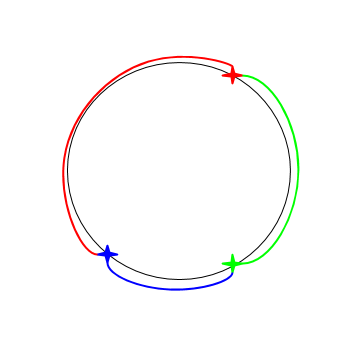
\includegraphics[width=0.5\linewidth]{figs/voro-chord-normal}
	\caption{A Voronoi diagram for a Chord network, using Chord's definition of closest.}
	\label{fig:voro-chord-normal}
\end{figure}

\begin{figure}
	\centering
	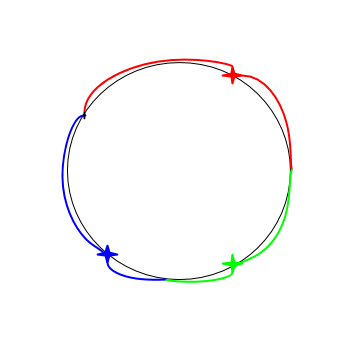
\includegraphics[width=0.5\linewidth]{figs/voro-chord-alternative}
	\caption{A Voronoi diagram for a Chord network, where closest is defined by the node being the closest in either direction.}
	\label{fig:voro-chord-alternative}
\end{figure}

 
\subsection{Terminology}
% % %unified terminology
The large number of DHTs have lead many papers to use different terms to describe congruent elements of DHTs, as some terms may make sense only in one context.
Since this paper will cover multiple DHTs that use different terms, we have created a unified terminology:


\begin{description}
    \item[key] -  The identifier generated by a hash function corresponding to a unique\footnote{Unique with extremely high probability.     The probability of a hash collision is extremely low and are ignored in most formal  specifications for DHTs.  This could be resolved for any file by using any number of the collision resolution strategies, such as chaining or linear probing.  However, resolving a collision of two nodes is much more problematic with no canonical solution other than praying it won't happen.} node or file.
    SHA-1, which generates 160-bit hashes, is typically used as a hashing algorithm.\footnote{Due to the research into hash collisions \cite{stevens2012attacks}, and the glut of hardware that currently exists to perform SHA hash collisions, SHA1 is being depreciated by many companies in 2017. This will undoubtedly lead to some kind of security flaw in a decade or so, when some entrepreneuring hacker figures out a way to force websites to accept a forged SHA1 key.}
    
	\item[ID] - The ID is a key that corresponds to a particular node.  
	The ID of a node and the node itself are referred to interchangeably.
	In this proposal, we refer to nodes by their ID and files by their keys.
	\item[Peer]  - Another active member on the network.
	For this section, we assume that all peers are different pieces of hardware.
	\item[Peerlist] -  The set of all peers that a node knows about. 
	This is sometimes referred to as the \textit{routing table}, but certain DHTs  \cite{pastry} \cite{tapestry}  overload the terminology.
	Any table or list of peers is a subset of the entire peerlist.
	\item[Short-hops] - The subset of peers that are ``closest/adjacent'' to the node in the keyspace, according to the DHT's metric.  
	In a 1-dimensional ring, such a Chord \cite{chord}, this is the node's \textit{predecessor(s)} and \textit{successor(s)}.
	They may also be called \textit{neighbors}.
	\item[Long-hops] - The subset of the peerlist that the node is not adjacent to.  
	These are sometimes referred to as fingers, long links, or shortcuts.
	\item[Root Node] - The node responsible for a particular key. 
	\item[Successor] -  Alternate name for the root node. 
	The successor of a node is the neighbor that will assume a nodes responsibilities if that node leaves. 
    \item[$n$ nodes] -  The number of nodes in the network.
    
\end{description}
Similarly, All DHTs perform the same operations with minor variation.
\begin{description}
	\item[\texttt{lookup(key)}] - This operation finds the root node of \texttt{key}.
	Almost every operation on a DHT needs to leverage the \texttt{lookup} operation in some way.
	\item[\texttt{put(key,value)}] - Stores \texttt{value} at the root node of \texttt{key}.
	Unless otherwise specified, \texttt{key} is assumed be the hashkey of \texttt{value}.
	This assumption is broken in Tapestry.
	\item[\texttt{get(key)}] - This operates like lookup, except the context is to return the value stored by a \texttt{put}.
	This is a subtle difference, since one could \texttt{lookup(key)} and ask the corresponding node directly.
	However, many implementations use backup operations and caching, which will store multiple copies of the value along the network.
	If we do not care which node returns the value mapped with \texttt{key}, or if it is a backup,  we can express it with \texttt{get}.
	\item[\texttt{delete(key, value)}] - This is self-explanatory.  Typically, DHTs do not worry about key deletion and leave that option to the specific application.
    When DHTs do address the issue, they often assume that stored key-value pairs have a specified time-to-live, after which they are automatically removed.
\end{description}

On the local level, each node has to be able to \textit{join }and perform maintenance on itself.
\begin{description}
	\item[\texttt{join()}]  The join process encompasses two steps.
    First, the joining node needs to initialize its peerlist. 
    It does not necessarily need a complete peerlist the moment it joins, but it must initialize one. 
    Second, the joining node needs to inform other nodes of its existence.
    \item[Maintenance]  Maintenance procedures generally are either \textit{active} or \textit{lazy}.
    In active maintenance, peers are periodically pinged and are replaced when they are no longer detected.
    Lazy maintenance assumes that peers in the peerlist are healthy until they prove otherwise, in which case they are either replaced immediately.
    In general, lazy maintenance is used on everything, while active maintenance is only used on neighbors\footnote{check this statement for consistency}.
    
\end{description}

When analyzing the DHTs in this chapter, we look at the overlay's geometry, the peerlist, the \texttt{lookup} function, and how fault-tolerance is performed in the DHTs.
We assume that nodes never politely leave the network but always abruptly fail, since a \texttt{leave()} operation is fairly trivial and has minimal impact.


\section{Chord}
%Chord \cite{chord} is a P2P protocol for file sharing and distributed storage that guarantees a high probability $\log_{2} n$ lookup time for a particular node or file in the network. 
%It is highly fault-tolerant to node failures and churn, the constant joining and leaving of nodes.  It scales extremely well and the network requires little maintenance to handle individual nodes.  



Chord \cite{chord} is the archetypal ring-based DHT and it is impossible to create a new ring-based DHT without making some comparison to Chord.
It is notable due its straightforward routing, its rules which make ownership of keys very easy to sort out, and the large number of derivatives.



% Should I put this in?
Chord is extremely well known in Computer Science, and was awarded the prestigious 2011 SIGCOMM Test of Time Award \cite{zave2012using}.
However, recent research has demonstrated that there have been no correct implementations of Chord in over a decade \cite{zave2012using}.




\subsection*{Peerlist and Geometry}
Chord is a 1-dimensional modular ring in which all messages travel in one direction - upstream, hopping from one node to another node with a greater ID until it wraps around.
Each member of the network and the data stored within it is hashed to a unique $m$-bit key or ID, corresponding to one of the $2^m$ locations on a ring. 
An example Chord network is shown in Figure \ref{fig:chord}.



\begin{figure}
	\centering
	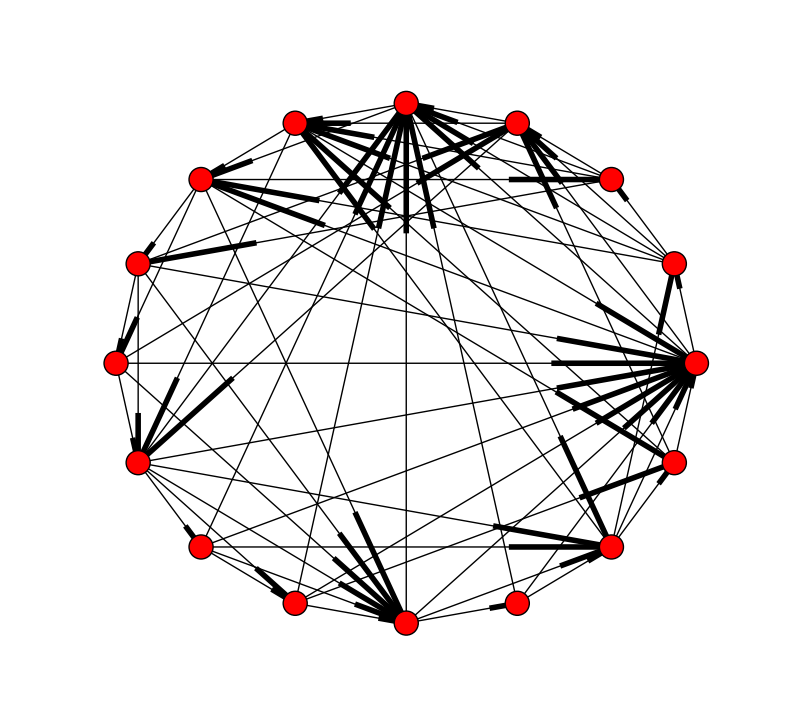
\includegraphics[width=0.45\linewidth]{figs/chord}
	\caption{A Chord ring with 16 nodes.  The fingers (long hop connections) are shown cutting across the ring.}
	\label{fig:chord}
\end{figure}



A node in the network is responsible for all the data with keys upstream from its predecessor's ID, up through and including its own ID.  
If a node is responsible for some key, it is referred to being the root or successor of that key.

Lookup and routing is performed by recursively querying nodes upstream.
Querying only neighbors in this manner would take $O(n)$ time to lookup a key.


To speedup lookups, each node maintains a table of $m$ shortcuts to other peers, called the \textit{finger table}.
The $i$th entry of a node $n$'s finger table corresponds to the node that is the successor of the key $n+2^{i-1} \mod 2^m $.  
During a lookup,  nodes query the finger that is closest to the sought key without going past it, until it is received by the root node.
Each hop essentially cuts the search space for a key in half.
This provides Chord with a highly scalable $\log_2(n)$ lookup time for any key \cite{chord}, with an average $\frac{1}{2}O(\log_{2}(n))$ number of hops.

Besides the finger tables, the peerlist includes a list of $s$ neighbors in each direction for fault tolerance.
This brings the total size of the peerlist to $log_{2}(2^{m})  + 2 \cdot s =  m  + 2 \cdot s$, assuming the entries are distinct.

\subsection*{Joining}
To join the network, node $n$ first asks $n'$ to find \texttt{successor($ n $)}. 
Node $n$ uses the information to set his successor, and maintenance will inform the other nodes of $n$'s existence.
Meanwhile, $n$ will takeover some of the keys that his successor was responsible for.

\subsection*{Fault Tolerance}
Robustness in the network is accomplished by having nodes backup their contents to their $s$ immediate successors, the closest nodes upstream. 
This is done because when a node leaves the or fail, the most immediate successor would be responsible for the keys.
In the case of multiple nodes failing all at once, having a successor list makes it extremely unlikely that any given stored value will be lost.

As nodes enter and leave the ring, the nodes use their maintenance procedures to guide them into the right place and repair any links with failed nodes.  
The process takes $O(\lg^{2}(n))$ messages.
Full details on Chord's maintenance cycle can be found here \cite{chord}.

%\subsection*{Security}
%An Eclipse attack compromises a DHT by poisoning the routing tables of nodes, such that friendly nodes can only communicate with malicious nodes \cite{dhtsec}.
%Because 





\section{Kademlia}
Kademlia \cite{kademlia}  is perhaps the most well known and most widely used DHT, as a modified version of Kademlia (Mainline DHT) is forms backbone of the BitTorrent protocol.
The motivation of Kademlia was to create a way for nodes to incorporate peerlist updates with each query made.

%(the security ramifications of gossip based routing tables being ignored, I suppose).

\subsection*{Peerlist and Geometry}
Like Chord, Kademlia uses $m$-bit keys for nodes and files.
However, Kademlia utilizes a binary tree-based structure, with the nodes acting as the leaves of the tree.
Distance between any two nodes in the tree  is calculated by XORing their IDs.
The XOR distance metric means that distances are symmetric, which is not the case in Chord.

%A node's location in the tree given by the shortest unique prefix of its ID.   
%For each bit in the prefix, there would be a subtree which does not contain that node.  
%Kademlia guarantees that the node will know at least one node in each of these subtrees.

Nodes in Kademlia maintain information about the network using a routing table that contains  $m$ lists, called $k$-buckets.
For each $k$-bucket contains up to $k$ nodes that are distance $2^i$ to $2^{i+1}$, where $0 \leq i < m$.
In other words, each $k$-bucket corresponds to a subtree of the network not containing the node.
An example network is shown in Figure \ref{fig:kademlia}.

\begin{figure}
	\centering
	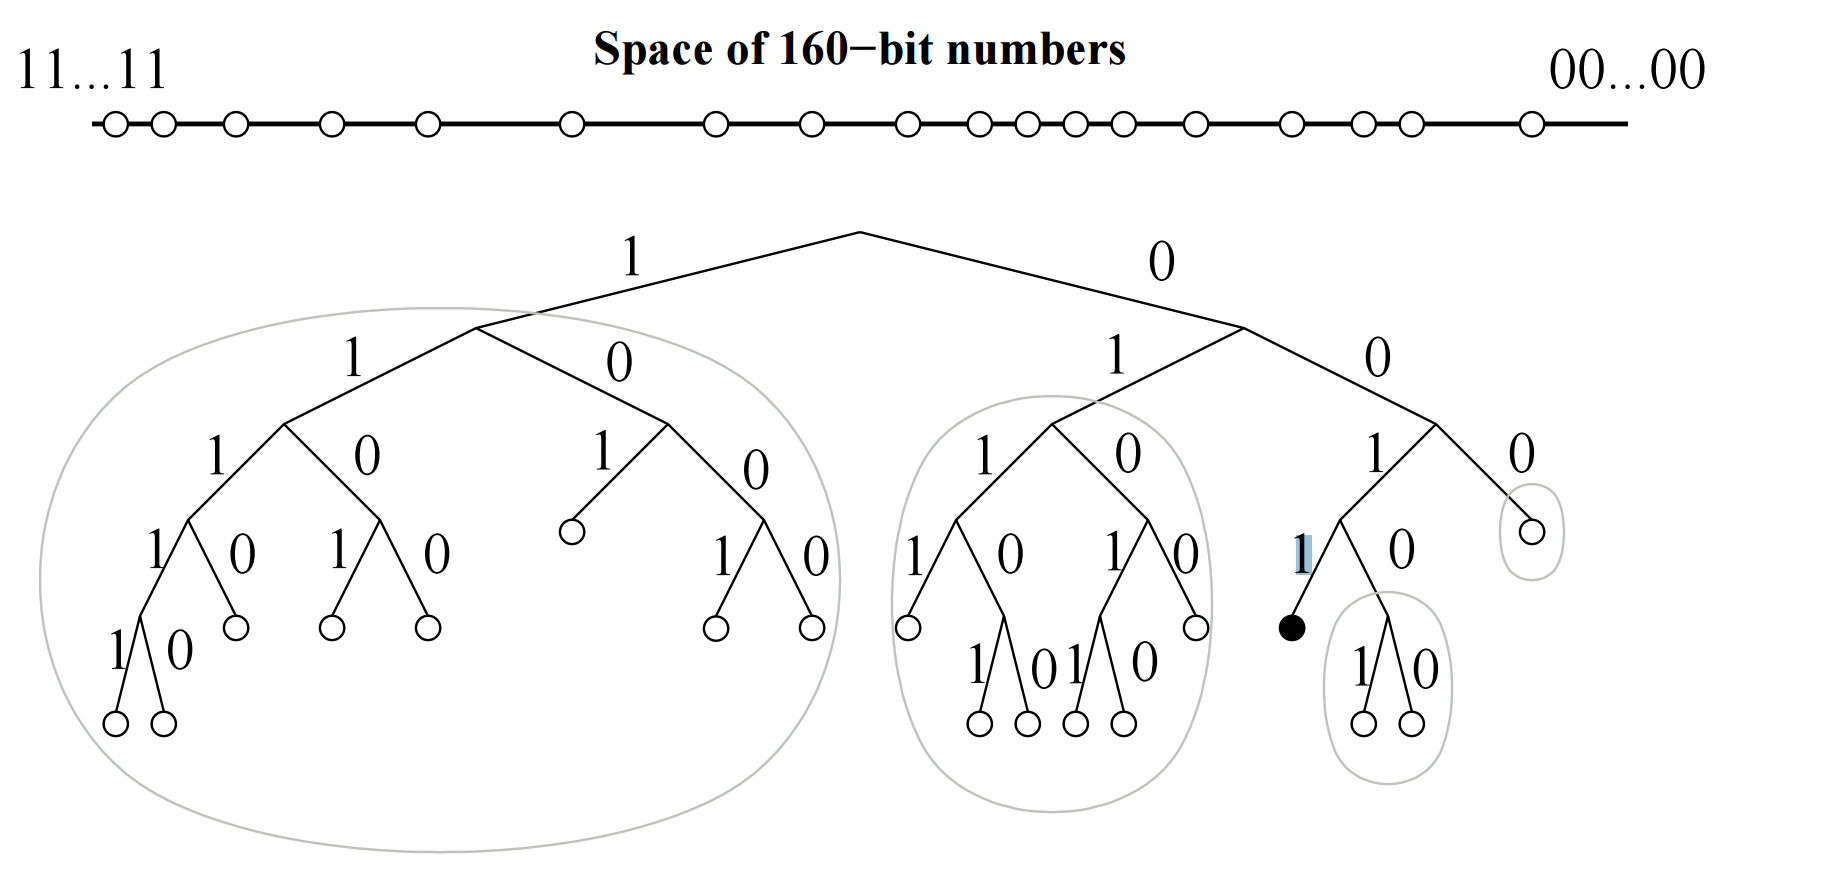
\includegraphics[width=0.7\linewidth]{figs/kademlia}
	\caption{An example Kademlia network from the original paper \cite{kademlia}. The ovals are the node's $k$-buckets.}
	\label{fig:kademlia}
\end{figure}




Each $k$-bucket is maintained by a least recently seen eviction algorithm that skips live nodes.
Whenever the node receives a message, it adds the sender's info to the tail of the corresponding $k$-bucket.
If that info already exists, the info is moved to the tail.

If the $k$-bucket is full, the node starts pinging nodes in the list, starting at the head.
As soon as a node fails to respond, that node is evicted from the list to make way for the new node at the tail.

If there are no modifications to a particular $k$-bucket after a long period of time, the node does a \texttt{refresh} on the $k$-bucket.
A refresh is a \texttt{lookup} of a random key in that $k$-bucket.


%(If I'm an eclipse attacker, I just keep spamming messages of different IDs, but with my own ip address and port info, or with sybils)

\subsection*{Lookup}
In most DHTs, \texttt{lookup(key)} sends a single message and returns the information  of a single node.
The \texttt{lookup} operation in Kademlia differs in both respects:  \texttt{lookup} is done in parallel and each node receiving  a \texttt{lookup(key)} returns the $k$ closest nodes to \texttt{key} it knows about.


A \texttt{lookup(key)} operation begins with the seeking node sending lookups in parallel to the $\alpha$ nodes from the appropriate $k$-bucket.
Each of theses $\alpha$ nodes will asynchronously return the $k$ closest nodes it knows closest to \texttt{key}.
As lookups return their results, the node continue to send lookups until no new nodes\footnote{If a file being stored on the network is the objective, the \texttt{lookup} will also terminate if a node reports having that file.} are found.  

\subsection*{Joining}
A joining node starts with a single contact and then performs a \textit{lookup} operation on its own ID.
Each step of the \textit{lookup} operation yields new nodes for the joining node's peerlist and informs other nodes of its existence.
Finally, the joining node performs a \texttt{refresh} on each $k$-bucket farther away than the closest node it knows of.




\subsection*{Fault-Tolerance}
Nodes actively republish each file stored on the network each hour by rerunning the \texttt{store} command.  
To avoid flooding the network, two optimizations are used.

First if a node receives a \texttt{store} on a file it is holding, it assumes $k-1$ other nodes got that same command and resets the timer for that file.
This means only one node republishes a file each hour.
Secondly, \texttt{lookup} is not performed during a republish.


Additional fault tolerance is provided by the nature of the \texttt{store(data)} operation, which \texttt{puts }the file in the $k$ closest nodes to the key.
However, there is very little in the way of frequent and active maintenance other than what occurs during \texttt{lookup} and the other operations.


%\subsubsection*{Caching}
%Files are cached during a \texttt{get} operation and stored at the closest node that the seeker found that did not return a result.
%The cache has an expiration 










\section{CAN}
%TODO: REREAD, APPARENTLY A COUPLE OF WAYS TO define NEIGHBORHOOD


Unlike the previous DHTs presented in this chapter, the Content Addressable Network (CAN) \cite{can} works in a $d$-dimensional torus, with the entire coordinate space divided among members.
A node is responsible for the keys  that fall within the ``zone'' that it owns.
Each key is hashed into some point within the geometric space.

\subsection*{Peerlist and Geometry}
CAN uses an exceptionally simple peerlist consisting only of neighbors.  
Every node in the CAN network is assigned a geometric region in the coordinate space and each node maintains a routing table consisting each node that borders the node's region.
An example CAN network is shown in Figure \ref{fig:can}


\begin{figure}
	\centering
	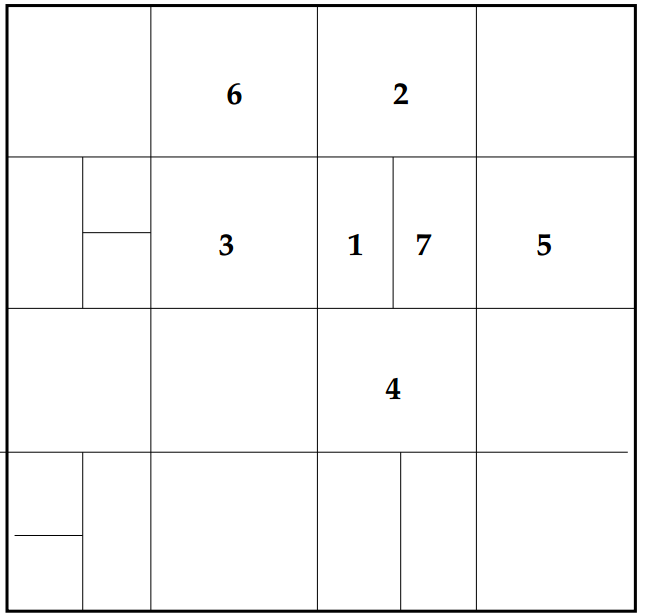
\includegraphics[width=0.7\linewidth]{figs/can}
	\caption{An example CAN network from \cite{can}.}
	\label{fig:can}
\end{figure}


The size of the routing table is a function of the number of dimensions, $O(d)$. 
The lower bound on the routing tables size in a populated network (eg, a network with at least $2d$ nodes) is $\Omega(2d)$.  
This is obtained by looking at each axis, where there is at least one node bordering each end of the axis.
The size of the routing table can grow as more nodes join and the space gets further divided; however, maintenance algorithms prevent the regions from becoming too fragmented.


\subsection*{Lookup}
As previously mentioned, each node maintains a routing table corresponding to their neighbors, those nodes it shares a face with.
Each hop forwards the lookup to the neighbor closest to the destination, until it comes to the responsible node.
In a space that is evenly divided among $n$ nodes, this simple routing scheme uses only $2 \cdot d$ space while giving average path length of $\frac{d}{4}\cdot n^{\frac{1}{d}}$.
The overall lookup time of in CAN is bounded by $O(n^{\frac{1}{d}})$ hops\footnote{Around the same time CAN was being developed, Kleinberg was doing research into small world networks \cite{kleinberg2000small}.  
He proved similar properties for lattice networks with a single shortcut.  What makes this network remarkable is lack of shortcuts.}.

% fault tolerence in routing
If a node encounters a failure during lookup, the node simply chooses the next best path.
However, if lookups occur before a node can recover from damage inflicted by churn, it is possible for the greedy lookup to fail.
The fallback method is to use an expanding ring search until a candidate is found, which recommences greedy forwarding.

\subsection*{Joining}
Joining works by splitting the geometric space between nodes.  
If node $n$ with location $P$ wishes to join the network, it contacts a member of the node to find the node $m$ currently responsible for location $P$.
Node $n$ informs $m$ that it is joining and they divide $m$'s region such that each becomes responsible for half.

Once the new zones have been defined, $n$ and $m$ create its routing table from $m$ and its former neighbors.
These nodes are then informed of the changes that just occurred and update their tables.
As a result, the join operation affects only $O(d)$ nodes.  
More details on this splitting process can be found in CAN's original paper \cite{can}.

\subsection*{Repairing}
A node in a DHT that notifies its neighbors that its leaves usually has minimal impact to the  network and in this is true for most cases in CAN.
A leaving node, $f$, simply hands over its zone to one of its neighbors of the same size, which merges the two zones together.
Minor complications occur if this is not possible, when there is no equally-sized neighbor. 
In this case, $f$ hands its zone to its smallest neighbor, who must wait for this fragmentation to be fixed.



Unplanned failures are also relatively simple to deal with.
Each node broadcasts a heartbeat to its neighbors, containing its and its neighbors' coordinates.
If a node fails to hear a heartbeat from $f$ after a number of cycles, it assumes $f$ must have failed and begins a \texttt{takeover} countdown.
When this countdown ends, the node broadcasts\footnote{This message is sent to all of $f$'s neighbors.} a \texttt{takeover} message in an attempt to claim $f$'s space.
This message contains the node's volume.
When a node receives a \texttt{takeover} message, it either cancels the countdown or, if the node's zone is smaller than the broadcaster's, responds with its own \texttt{takeover}.

The general rule of thumb for node failures in CAN is that the neighbor with the smallest zone takes over the zone of the failed node.
This rule leads to quick recoveries that affect only $O(d)$ nodes, but requires a zone reassignment algorithm to remove the fragmentation that occurs from \texttt{takeovers}.

To summarize, a failed node is detected almost immediately, and recovery occurs extremely quickly, but fragmentation must be fixed by a maintenance algorithm.




%As mentioned earlier in the text, Ratnasamy et al. \cite{can}  also present the concept own using landmarks to choose coordinates, rather than a has function.
%Each node measures the round-trip time (RTT) to each to of the $m$ landmarks, which yields one of $m!$ permutations.
%The keyspace is partitioned into $m!$ regions, each corresponding to one of the orderings.  
%A joining node now chooses a random location from the region corresponding to its landmark ordering.






%\subsection*{Design Improvements}
%Ratnasamy et al.\ identified a number of improvements that could be made to CAN \cite{can}.
%Some of these improvements have already be explored in Chapter 1.

%One modification to the system is increasing the number of dimensions in the coordinate space.
%Increasing $d$ improves fault tolerance and reduces path length.

%One concept Ratnasamy et al.\  introduces is the idea of multiple coordinate spaces existing simultaneously, called \textit{realities}. 
%Each object in the DHT exists at a different set of coordinates for each reality simultaneously.
%So a node might have coordinates $(x_0,y_0,z_0)$ in one reality, while having coordinates $(x_1,y_1,z_1)$ in another.
%Independent sets of neighbors for each reality yield different the overall topologies and mappings of keys to nodes.
%Multiple realities increase the cost of maintenance and routing table sizes, but provide greater fault tolerance and greater data availability.

%A final modification is to allow multiple nodes shares the same zone (ie zones don't necessarily split as a result of a join operation).    


\section{Pastry}

%Addressing - 128 bit ID, 0 to $2^{128} -1$, assigned randomly using hash.   but thought of as base $2^{b}$ numbers (typically b=4).  
Pastry \cite{pastry} and Tapestry \cite{tapestry} are extremely similar use a prefix-based routing mechnism introduced by Plaxton et al.\ \cite{plaxton1999accessing}.
In Pastry and Tapestry, each key is encoded as a base $ 2^{b} $ number (typically $b=4$ in Pastry, which yields easily readable hexadecimal).
The resulting peerlist best resembles a hypercube topology \cite{induced}, with each node being a vertice of the hypercube.

One notable feature of Pastry is the incorperation of a proximity metric.
The peerlist uses IDs that are close to the node according to this metric.

\subsection*{Peerlist}
Pastry's peerlist consists of three components: the routing table, a leaf set, and a neighborhood set.  
The routing table consists of $\log_{2^{b}}(n)$ rows with $2^{b} -1 $ entries per row. 
The $i$th level of the routing table correspond to the peers with that match first $i$ digits of the example nodes ID.

Thus, the 0th row contains peers which don't share a common prefix with the node, the 1st row contains those that share a length 1 common prefix, the 2nd a length 2 common prefix, etc.  
Since each ID is a base $2^b$ number, there is one entry for each of the $2^{b} -1 $ possible differences.   

For example, let is consider a node 05AF in system where $b = 4$ and the hexadecimal keyspace ranges from $0000$ to FFFF.
\begin{itemize}
    \item 1322 would be an appropriate peer for the 1st entry of level 0.
    \item 0AF2 would be an appropriate peer for the 10th\footnote{0 is the 0th level.} entry of level 1.
    \item 09AA would be an appropriate peer for the 9th entry of level 1.	
    \item 05F2 would be an appropriate peer for the 2nd entry of level 3.
\end{itemize}


The leaf set is used to hold the $L$ nodes with the numerically closest IDs;  half of it for smaller IDs and half for the larger.
A typical value for $L$ is $2^b$ or $2^{b+1}$.
The leaf set is used for routing when the destination key is close to the current node's ID.
The neighborhood set contains the $L$ closest nodes, as defined by some proximity metric.  
It, however, is generally not used for routing.  
Figure \ref{fig:pastry-table} shows an example peerlist of a node in PAST.

\begin{figure}
	\centering
	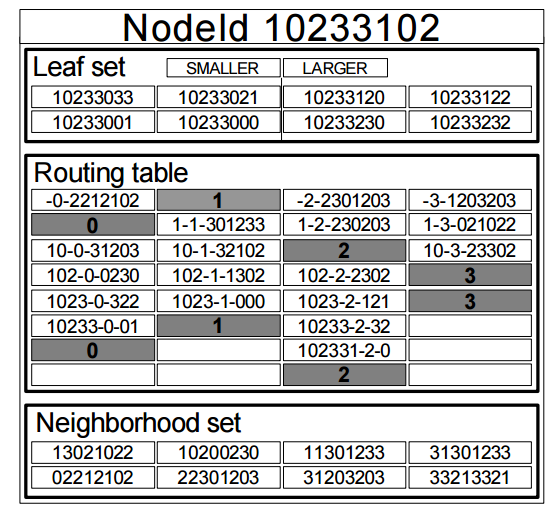
\includegraphics[width=0.5\linewidth]{figs/pastry-table}
	\caption{An example peerlist for a node in Pastry \cite{pastry}.}
	\label{fig:pastry-table}
\end{figure}



\subsection*{Lookup}
The \texttt{lookup} operation is a fairly straightforward recursive operation.
The \texttt{lookup(key)} terminates when the \texttt{key} is falls within the range of the leaf set, which are the nodes \emph{numerically} closest to the current node.
In this case, the destination will be one of the leaf set, or the current node.

If the destination node is not immediately apparent, the node uses its routing table to select the next node.
The node looks at the length $l$ shared prefix,  at examines the $l$th row of its routing table.
From this row, the \texttt{lookup} continues with the entry that matches at least another digit of the prefix.
In the case that this entry does not exist or has failed, the \texttt{lookup} continues from the closest ID chosen from the entire peerlist.
This process is described by Algorithm \ref{PastryLookup}.
Lookup is expected  to take $\lceil \log_{2^{b}} \rceil $, as each hop along the routing table reduces the search space by $\frac{1}{2^{b}}$.
 
\begin{algorithm}
    \caption{Pastry lookup algorithm}
    \label{PastryLookup}
    \begin{algorithmic}
        \State Let $L$ be the routing  
        \Function{Lookup}{$key$}
            \If {$key$ is in the range of the leaf set }
            	\State destination is closest ID in the leaf set or self
            \Else
            	\State $next\gets$ entry from routing table that matches $\geq 1$ more digit
            	\If {$next \neq null$}
                	\State forward to $next$
            	\Else
                	\State forward to the closest ID from the entire peerlist
                \EndIf
                
            \EndIf
        \EndFunction
    \end{algorithmic}
\end{algorithm}

\subsection*{Joining}
To join the network, node $J$ sends a \texttt{join} message to $A$, some node that is close according to the proximity metric.
The \texttt{join} message is forwarded along like a \texttt{lookup} to the root of $X$, which we'll call $root$.
Each node that received the \texttt{join} sends a copy of the their peerlist to $J$.

The leaf set is constructed from copying $root$'s leaf set, while $i$th row in the routing table routing table is copied from the $i$th node contacted along the \texttt{join}.
The neighborhood set is copied from $A$'s neighborhood set, as \texttt{join} predicates that $A$ be close to $J$.
This means $A$'s neighborhood set would be close to $A$. 

After the joining node creates its peerlist, it sends a copy to each node in the table, who then can update their routing tables.  
The cost of a \texttt{join} is $O(log_{2}^{b} n)$ messages,  with  a constant  coefficient  of $3*2^{b}$




\subsection*{Fault Tolerance}
Pastry lazily repairs its leaf set and routing table.
When node from the leaf set fails, the node contacts the node with largest or smallest ID (depending if the failed node ID was smaller or larger respectively) in the leaf set.
That node returns a copy of its leaf set, and the node replaces the failed entry.
If the failed node is in the routing table, the node contacts a node with an entry in the same row as the failed node for a replacement.

Members of the neighborhood set are actively checked.
If a member of the neighborhood set is unresponsive, the node obtains a copy of another entry's neighborhood set and repairs from a selection.



%\subsection*{Proximity Metric}
%Pastry's goal is to minimize the ``distance'' messages travel, where distance can be defined by some metric, typically the number of hops.
%The leaf set is the  of nodes closest to the node in the keyspace.  
%The neighborhood set is the of nodes closest to the node according to the distance metric. 
%Guarantees routing time is  $<\log n$ in typical operation.  
%Guarantees eventual delivery except when half of the leaf nodes fail simultaneously.






%\section{Tapestry}
%Tapestry \cite{tapestry} is based off the same prefix-based lookup \cite{prr} as Pastry \cite{pastry} and the peerlist and lookup operation share many similarities.
%Tapestry views itself more as a DOLR \cite{dolr}.
%This essentially means that it is a distributed key-based lookup system like a DHT \cite{hildrum2004distributed}, but with some subtle differences at the abstract level which manifest as large %implementation changes.
%The essential difference here is that Tapestry has servers \textit{publish} records/objects on the network, which direct lookups to the server.  
%The assumption here seems to be that the servers, not the responsible node, serve the actual data.  
%DHTs care or don't care on an application to application basis whether keys are associated with records or content. 






% ``Small'' routing tables
\section{Symphony and Small World Routing}
Symphony  \cite{symphony} is a 1$d$ ring-based DHT similar to Chord \cite{chord}, but is constructed using the properties of small world networks \cite{kleinberg2000small}.
Small world networks owe their name to a phenomena observed by psychologists in the late 1960's. 

Subjects in experiments were to route a postal message to a target person; for example the wife of a Cambridge divinity student in one experiment and a Boston stockbroker in another \cite{milgram1967small}.
The messages were only to be routed by forwarding them to a friend they thought most likely to know the target.
Of the messages that successfully made their way to the destination, the average path length from a subject to a participant was only 5 hops.  

This lead to research investigating creating a network with randomly distributed links, but with a efficient lookup time.
Kleinberg \cite{kleinberg2000navigation} showed that in a 2-dimensional lattice network, nodes could route messages in $O(\log^{2}n)$ hops using only their neighbors and a single randomly chosen\footnote{Randomly chosen from a specified distribution.} finger.
In other words, $O(\log^{2}n)$ lookup is achievable with a $O(1)$ sized routing table.

\subsection*{Peerlist}
Rather than the 2-dimensional lattice used by Kleinberg, Symphony uses a 1-dimensional ring\footnote{This is technically a 1-dimensional lattice.} like Chord.
Symphony assigns $m$-bit keys to the modular unit interval $ [0,1)$, instead of using a keyspace ranging from 0 to $2^{n} - 1$.
This location is found  with $\frac{hashkey}{2^{m}}$.
This is arbitrary from a design standpoint, but makes choosing from a random distribution simpler. 

Nodes know both their immediate predecessor and successor, much like in Chord.
Nodes also keep track of some  $k \geq 1$ fingers, but, unlike in Chord, these fingers are chosen at random.
These fingers are chosen from a probability distribution corresponding to the expression $e^{ln(n) + (rand48() - 1.0)}$, where $n$ is the number of nodes in the network and \texttt{rand48()} is a C function that generates a random float?double between 0.0 and 1.0.
Because $n$ os difficult to compute due to the changing nature of P2P networks, each node uses an approximation is used based on the distance between themselves and their neighbors.

A final feature of note is that links in Symphony are bidirectional.
Thus, if a node creates a finger to a peer, that peer creates a, so nodes in Symphony have a grand total of $2k$ fingers.
%(although it gets me thinking, is there any advantage/statistical properties   that could be exploited by making the space monic)


\subsection*{Joining and Fault Tolerance}
The joining and fault tolerance processes in Symphony are extremely straightforward.
After determining its ID, a joining node asks a member to find the root node for its ID.
The joining node integrates itself in between its predecessor and successor and then randomly generates its fingers.

Failures of immediate neighbors are handled by use of successor and predecessor lists
Failures for fingers are handled lazily and are replaced by another randomly generated link when a failure is detected.

% Large Routing Tables
\section{ZHT}
One of the major assumptions of DHT design is that churn is a significant factor, which requires constant maintenance to handle.
A consequence of this assumption is that nodes only store a small subset of the entire network to route to.
Storing the entire network is not scalable for the vast majority of distributed systems due to bandwidth constraints and communication overhead incurred by the constant joining and leaving of nodes.

In a system that does not expect churn, the memory and bandwidth costs for each node to keep a full copy of the routing table are minimal.
An example of this would be a data center or a cluster built for higher-performance computing, where churn would overwhelmingly be the result of hardware failure, rather than users quitting.

ZHT \cite{li2013zht} is an example of such a system, as is Amazon's Dynamo \cite{dynamo}.
ZHT is a ``zero-hop hash table,'' which takes advantage of the fact that  nodes in  High-End Computing environments have a predictable lifetime.
Nodes are created when a job begins and are removed when a job ends.
This property allows ZHT to \texttt{lookup} in $ O(1) $ time.

\subsection*{Peerlist}

ZHT operates in a 64-bit ring, for a total of $N = 2^{64}$ addresses.
ZHT places a  hard limit of $ n $ on the maximum number of physical nodes in the network, which means the network has $n$ partitions of $\frac{N}{n} =  \frac{2^{64}}{n}$ keys.
The partitions are evenly divided along the network.

The network consists of $k$ physical nodes which each are running at least one instance (virtual nodes) of ZHT, with a combined total of $i$ .
Each instance is responsible for some span of partitions in the ring.


Each node maintains a complete list of all nodes in the network, which do not have to be updated very often due to the lack of or very low levels of churn.
The memory cost is extremely low.
Each instance has a 10MB footprint, and each entry for the membership table takes only 32 bytes per node.
This means routing takes anywhere between 0 to 2 hops (explained below).

\subsection*{Joining}
ZHT operates under a static or dynamic membership.
In a static membership, no nodes will be joining the network once the network has been bootstrapped.
Nodes can join at any time when ZHT is using dynamic membership.

To join, the joiner asks a random member for a copy of the peerlist 
The joiner can then determine which node is the most heavily overloaded.
The joiner chooses an address in the network to take over partitions from that node.

\subsection*{Fault Tolerance}
Fault tolerance exists to handle only hardware failure or planned departures from the network.
Nodes backup their data to their neighbors.

\section{Summary}
% % % table
% Perhaps geometries should be included?
% be sure to include join and leave costs.

We have seen that there are a wide variety of distributed hash tables, but they have some clearly defined characteristics that bind them all together.
Table \ref{tab:tradeoffs} summarizes the information presented in this chapter.


\begin{table}[h]
	\tiny
	\centering
	\begin{tabularx}{\textwidth}{ |X|X|X|X|X| }
		\hline
		% Add join leave cost, avgerages and maxs
		DHT & Routing Table Size & Lookup Time & Join/Leave & Comments \\ \hline  
		
		Chord \cite{chord} & $O(\log n)$, maximum $m +2s$ & $O(\log n)$, avg $(\frac{1}{2} \log n)$  &  $<O(\log n^{2})$ total messages& $m$  = keysize in bits, $s$ is neighbors in 1 direction  \\ \hline
		
		Kademlia \cite{kademlia} & $O(\log n)$, maximum $m\ \cdot k$ & $(\lceil \log n\rceil) + c$ & $O(\log(n))$& This is without considering optimization   \\ \hline
		CAN \cite{can} & $\Omega(2d)$ & $O(n^{\frac{1}{d}})$, average $\frac{d}{4}\cdot n^{\frac{1}{d}}$ & Affects $O(d)$ nodes & $d$ is the number of dimensions \\ \hline
		
		Plaxton-based DHTs, Pastry \cite{pastry}, Tapestry \cite{tapestry} & $O(\log_{\beta} n)$ & $ O(\lceil \log_{2^{\beta}} \rceil) $ & $O(\log_{\beta} n)$ &  NodeIDs are base $\beta$ numbers \\ \hline
		
        Symphony \cite{symphony}& $2k + 2$&   average $O(\frac{1}{k} \log^{2} n )$ & $O(\log^{2} n)$ messages,  constant $<1$ &  $k \geq 1$, fingers are chosen at random\\ \hline  
		
        ZHT \cite{li2013zht}&   $O(n)$& $O(1)$ &  $O(n)$ & Assumes an extremely low churn \\ \hline
        
        VHash & $\Omega(3d+1) + O((3d+1)^{2})$ & $O(\sqrt[d]{n})$ hops & $3d + 1$ & approximates regions, hops are based least latency\\ \hline
	\end{tabularx}
	\caption{The different ratios and their associated DHTs}
	\label{tab:tradeoffs}
\end{table}

% % % Specific DHTs




	%\chapter{Completed Work}
\label{chapter:prev}

In this chapter, we will cover our completed research.
Our research has focused on novel implementation ]and Distributed Hash Tables (DHTs).
We have implemented and created an entirely new DHT called VHash \cite{vhash}, implemented MapReduce on Chord \cite{chordreduce}, and performed an analysis on an attack on DHTs.


\section{VHash}
DHTs all seek to minimize lookup time for their respective topologies.
This is done by minimizing the number of overlay hops needed for a lookup operation.
This is a good approximation for minimizing the latency of lookups, but does not actually do so, as each hop has a different amount of latency.
Furthermore, a network might need to minimize some arbitrary metric, such as energy consumption.

VHash is a multi-dimensional DHT that minimizes routing over some given metric.
It uses a fast approximation of a Delaunay Triangulation to compute the Voronoi tessilation of a multi-dimensional space.
%Approximated routing tables



Arguably all Distributed Hash Tables (DHTs) are built on the concept of Voronoi tessellations.
In all DHTs, a node is responsible for all points in the overlay to which it is the ``closest'' node.
Nodes are assigned a key as their location in some keyspace, based on the hash of certain attributes.
Normally, this is just the hash of the IP address (and possibly the port) of the node \cite{chord} \cite{kademlia} \cite{can} \cite{pastry}, but other metrics such as geographic location can be used as well \cite{ratnasamy2002ght}.

These DHTs have carefully chosen metric spaces such that these regions are very simple to calculate.
For example, Chord \cite{chord} and similar ring-based DHTs \cite{symphony} utilize a unidirectional, one-dimensional ring as their metric space, such that the region for which a node is responsible is the region between itself and its predecessor.

Using a Voronoi tessellation in a DHT generalizes this design.
Nodes are Voronoi generators at a position based on their hashed keys.
These nodes are responsible for any key that falls within its generated Voronoi region.

Messages get routed along links to neighboring nodes.
This would take $O(n)$ hops in one dimension.
In multiple dimensions, our routing algorithm (Algorithm \ref{alg:lookup}) is extremely similar to the one used in Ratnasamy et al.'s Content Addressable Network (CAN) \cite{can}, which would be $O(n^{\frac{1}{d}})$ hops.


\begin{algorithm}
	\caption{Lookup in a Voronoi-based DHT}
	\label{alg:lookup}
	\begin{algorithmic}[1]
		\State Given node $n$
		\State Given $m$ is a message addressed for $loc$
		\State $potential\_dests \leftarrow n \cup n.short\_peers \cup n.long\_peers$
		\State $c \leftarrow $ node in $ potential\_dests$ with shortest distance to $loc$
		\If{$c$ == $n$}
			\State \Return $n$
		\Else
			\State \Return $c.lookup(loc)$
		\EndIf
	\end{algorithmic}
\end{algorithm}


Efficient solutions, such as Fortune's sweepline algorithm \cite{fortune1987sweepline}, are not usable in spaces with 2 more dimensions.
As far as we can tell, there is no way efficient to generate higher dimension Voronoi tessellations, especially in the distributed Churn-heavy context of a DHT.
Our solution is the Distributed Greedy Voronoi Heuristic.

\subsection*{Distributed Greedy Voronoi Heuristic}
A Voronoi tessellation is the partition of a space into cells or regions along a set of objects $O$, such that all the points in a particular region are closer to one object than any other object.
We refer to the region owned by an object as that object's Voronoi region.
Objects which are used to create the regions are called Voronoi generators.
In network applications that use Voronoi tessellations, nodes in the network act as the Voronoi generators.

The Voronoi tessellation and Delaunay triangulation are dual problems, as an edge between two objects in a Delaunay triangulation exists if and only if those object's Voronoi regions border each other.
This means that solving either problem will yield the solution to both.
An example Voronoi diagram is shown in Figure \ref{voro-ex}.
For additional information, Aurenhammer \cite{voronoi} provides a formal and extremely thorough description of Voronoi tessellations, as well as their applications.


\begin{figure}
	\centering
	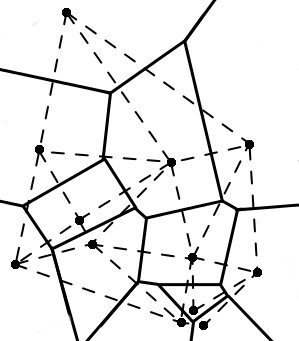
\includegraphics[width=0.5\linewidth]{figs/voronoi}
	\caption{An example Voronoi diagram for objects on a 2-dimensional space.  The black lines correspond to the borders of the Voronoi region, while the dashed lines correspond to the edges of the Delaunay Triangulation.}
	\label{voro-ex}
\end{figure}




The Distributed Greedy Voronoi Heuristic (DGVH) is a fast method for nodes to define their individual Voronoi region (Algorithm \ref{alg:dgvh}).
This is done by selecting the nearby nodes that would correspond to the points connected to it by a Delaunay triangulation.
The rationale for this heuristic is that, in the majority of cases, the midpoint between two nodes falls on the common boundary of their Voronoi regions.

%In addition, nodes should only have to compute their own Voronoi region, and possibly estimate those of its neighbors.
%Anything else is a waste of processing power.



\begin{algorithm} % make smaller
	\caption{Distributed Greedy Voronoi Heuristic}
	\label{alg:dgvh}
	\begin{algorithmic}[1]  % the numberis how many lines
		\State Given node $n$ and its list of $candidates$.
		\State Given the minimum $table\_size$
		\State $short\_peers \leftarrow$ empty set that will contain $n$'s one-hop peers
		\State $long\_peers \leftarrow$ empty set that will contain $n$'s two-hop peers
		\State Sort $candidates$ in ascending order by each node's distance to $n$
		\State Remove the first member of $candidates$ and add it to $short\_peers$
		\ForAll{$c$ in $candidates$}
		\State $m$ is the midpoint between $n$ and $c$
		\If{Any node in $short\_peers$ is closer to $m$ than $n$}
		\State Reject $c$ as a peer
		\Else
		\State Remove $c$ from $candidates$
		\State Add $c$ to $short\_peers$
		\EndIf
		\EndFor
		\While{$|short\_peers| < table\_size$ \textbf{and} $|candidates| >0$}
		\State Remove the first entry $c$ from $candidates$
		\State Add $c$ to $short\_peers$
		\EndWhile
		\State Add $candidates$ to the set of $long\_peers$
		\If{$|long\_peers| > table\_size^2$}
		\State $long\_peers \leftarrow$ random subset of $long\_peers$ of size $table\_size^2$
		\EndIf
	\end{algorithmic}
\end{algorithm}


During each cycle, nodes exchange their peer lists with a current neighbor and then recalculate their neighbors.
A node combines their neighbor's peer list with its own to create a list of candidate neighbors.
This combined list is sorted from closest to furthest.
A new peer list is then created starting with the closest candidate.
The node then examines each of the remaining candidates in the sorted list and calculates the midpoint between the node and the candidate.
If any of the nodes in the new peer list are closer to the midpoint than the candidate, the candidate is set aside.
Otherwise the candidate is added to the new peer list.


DGVH never actually solves for the actual polytopes that describe a node's Voronoi region.
This is unnecessary and prohibitively expensive \cite{raynet}.
Rather, once the heuristic has been run, nodes can determine whether a given point would fall in its region.

Nodes do this by calculating the distance of the given point to itself and other nodes it knows about.
The point falls into a particular node's Voronoi region if it is the node to which it has the shortest distance.
This process continues recursively until a node determines that itself to be the closest node to the point.
Thus, a node defines its Voronoi region by keeping a list of the peers that bound it.



\subsubsection{Algorithm Analysis}

DVGH is very efficient in terms of both space and time.
Suppose a node $n$ is creating its short peer list from $k$ candidates in an overlay network of $N$ nodes.
The candidates must be sorted, which takes $O(k\cdot\lg(k))$ operations.
Node $n$ must then compute the midpoint between itself and each of the $k$ candidates.
Node $n$ then compares distances to the midpoints between itself and all the candidates.
This results in a cost of

\[ k\cdot\lg(k) + k \text{ midpoints}  + k^{2} \text{ distances} \]


Since $k$ is  bounded by $\Theta(\frac{\log N}{\log \log N} )$ \cite{bern1991expected} (the expected maximum degree of a node), we can translate the above to

\[O(\frac{\log^{2} N}{\log^{2} \log N} )\]

In the vast majority of cases, the number of peers is equal to the minimum size of \textit{Short Peers}.
This yields $k=(3d+1)^{2}+3d+1$ in the expected case, where the lower bound and expected complexities are $\Omega(1)$.



\subsection{Experimental Results}
We evaluated the effectiveness of VHash and DGVH in creating a set of experiments.\footnote{Our results are pulled directly from \cite{dgvh} and \cite{vhash}.}
The first experiment showed how VHash could use DGVH to create a routing mesh.
Our second showed how optimizing for latency yielded better results than optimizing for least hops.

\subsubsection{Convergence}
Our first experiment examined how DGVH could be used to create a routing overlay and how well it performed in this task.
The simulation demonstrated how DGVH  formed a stable overlay from a chaotic starting topology after a number of cycles.
We compared our results to those in RayNet \cite{raynet}.
The authors of Raynet proposed a random $k$-connected graph would be a challenging initial configuration for showing a DHT relying on a gossip mechanism could converge to a stable topology.

In the initial two cycles of the simulation, each node bootstrapped its short peer list by appending 10 nodes, selected uniformly at random from the entire network.
In each cycle, the nodes gossiped , swapping peer list information.
They then ran DGVH using the new information.
We calculated the hit rate of successful lookups by simulating 2000 lookups from random nodes to random locations, as described in Algorithm \ref{alg:routesim}.
A lookup was considered successful if the network was able to determine which Voronoi region contained a randomly selected point.

Our experimental variables for this simulation were the number of nodes in the DGVH generated overlay and the number of dimensions.
We tested network sizes of 500, 1000, 2000, 5000, and 10000 nodes each in 2, 3, 4, and 5 dimensions.
The hit rate at each cycle is $\frac{hits}{2000}$, where $hits$ are the number of successful lookups.




\begin{algorithm}
	\caption{Routing Simulation Sample}
	\label{alg:routesim}
	\begin{algorithmic}[1]  % the number is how many
		\State $start \leftarrow$ random node
		\State$dest \leftarrow$ random set of coordinates
		\State $ans \leftarrow$ node closest to $dest$
		\If {$ans == start.lookup(dest)$}
		\State increment $hits$
		\EndIf
	\end{algorithmic}
\end{algorithm}

The results of our simulation are shown in Figure \ref{fig:conv}.
Our graphs show that a correct overlay was quickly constructed from a random configuration and that our hit rate reached 90\% by cycle 20, regardless of the number of dimensions.
Lookups consistently approached a hit rate of 100\% by cycle 30.
In comparison, RayNet's routing converged to a perfect hit rate at around cycle 30 to 35 \cite{raynet}.
As the network size and number of dimensions each increase, convergence slows, but not to a significant degree.

\begin{figure*}
	\centering
	\begin{tabular}{cc}

		\begin{subfigure}{0.5\columnwidth}
			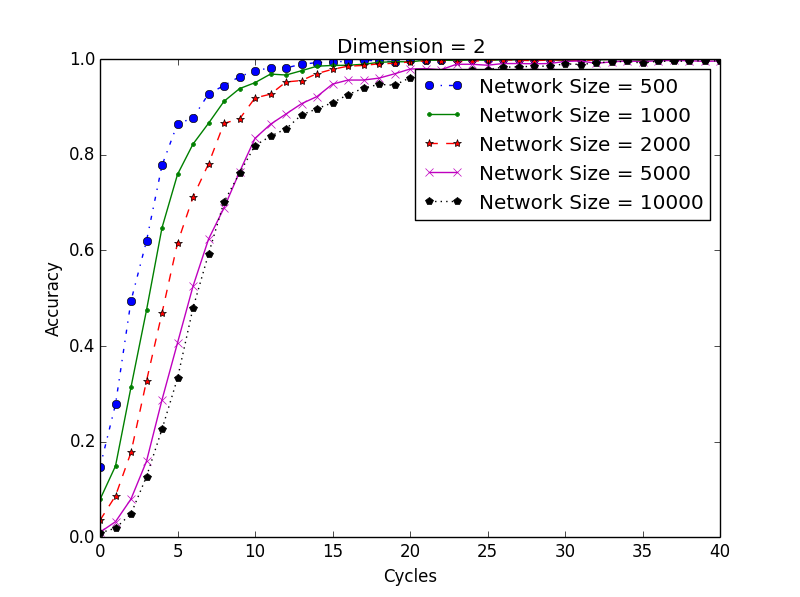
\includegraphics[width=\linewidth]{figs/conv_d2}
			\caption{This plot shows the accuracy rate of lookups on a 2-dimensional network as it self-organizes.}
			\label{fig:conv2}
		\end{subfigure} &

		\begin{subfigure}{0.5\columnwidth}
			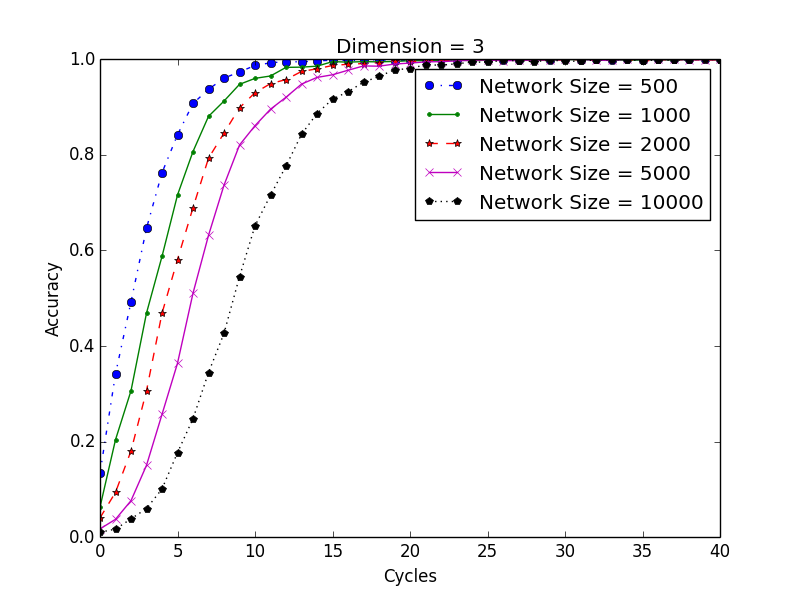
\includegraphics[width=\linewidth]{figs/conv_d3}
			\caption{This plot shows the accuracy rate of lookups on a 3-dimensional network as it self-organizes.}
			\label{fig:conv3}
		\end{subfigure} \\

		\begin{subfigure}{0.5\columnwidth}
			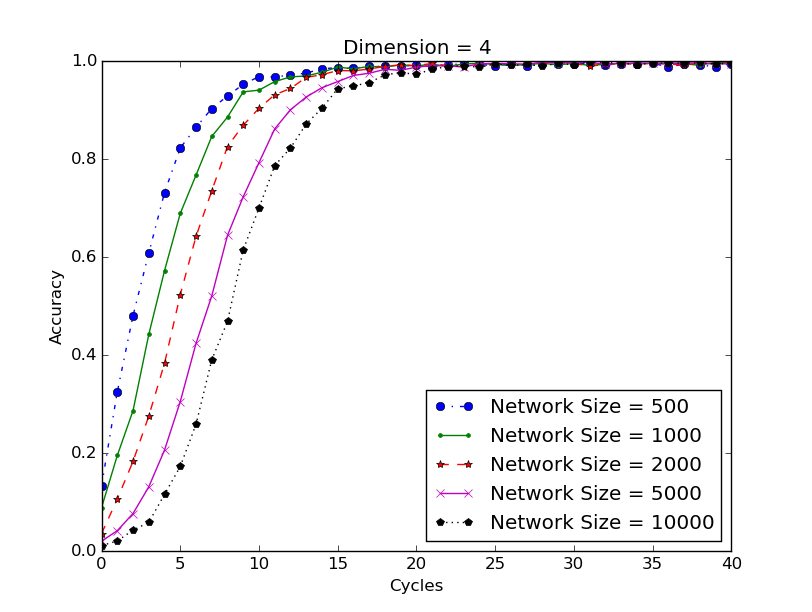
\includegraphics[width=\linewidth]{figs/conv_d4}
			\caption{This plot shows the accuracy rate of lookups on a 4-dimensional network as it self-organizes.}
			\label{fig:conv4}
		\end{subfigure} &


		\begin{subfigure}{0.5\columnwidth}
			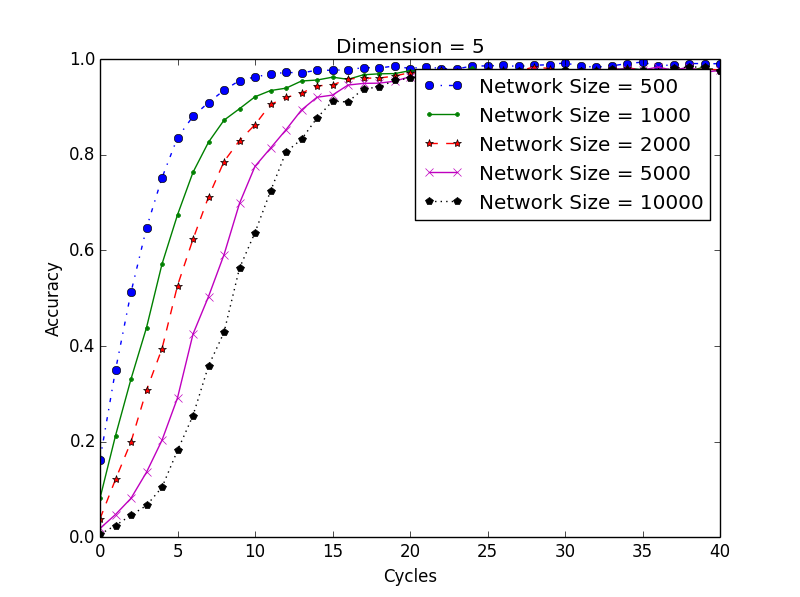
\includegraphics[width=\linewidth]{figs/conv_d5}
			\caption{This plot shows the accuracy rate of lookups on a 5-dimensional network as it self-organizes.}
			\label{fig:conv5}
		\end{subfigure}

	\end{tabular}
	\caption{These figures show that, starting from a randomized network, DGVH forms a stable and consistent network topology.
		The Y axis shows the success rate of lookups and the X axis show the number of gossips that have occurred.
		Each point shows the fraction of 2000 lookups that successfully found the correct destination.}
	
	\label{fig:conv}

\end{figure*}

\subsubsection{Latency Distribution Test}
The goal of our second set of experiments was to demonstrate VHash's ability to optimize a selected network metric: latency in this case.
In our simulation, we used the number of hops on the underlying network as an approximation of latency.
We compared VHash's performance to Chord \cite{chord}.
As we discussed in Chapter \ref{chapter:background} Chord is a well established DHT with an $O(\log(n))$ sized routing table and $O(\log(n))$ lookup time measured in overlay hops.

Instead of using the number of hops on the overlay network as our metric, we are concerned with the actual latency lookups experience traveling through the \emph{underlay} network, the network upon which the overlay is built.
Overlay hops are used in most DHT evaluations as the primary measure of latency.
It is the best approach available when there are no means of evaluating the characteristics of the underlying network.
VHash is designed with a capability to exploit the characteristics of the underlying network.
With most realistic network sizes and structures, there is substantial room for latency reduction in DHTs.

For this experiment, we constructed a scale free network with 10000 nodes placed at random (which has an approximate diameter of 3 hops) as an underlay network \cite{cohen2000resilience} \cite{pastor2001epidemic} \cite{hagberg2004}.
We chose to use a scale-free network as the underlay, since  scale free networks model the Internet's topology \cite{cohen2000resilience} \cite{pastor2001epidemic}.
We then chose a random subset of nodes to be members of the overlay network.
Our next step was to measure the distance in underlay hops between 10000 random source-destination pairs in the overlay.
VHash generated an embedding of the latency graph utilizing a distributed force directed model, with the latency function defined as the number of underlay hops between it and its peers.

Our simulation created 100, 500, and 1000 node overlays for both VHash and Chord.
We used 4 dimensions in VHash and a standard 160 bit identifier for Chord.




\begin{figure}

\begin{subfigure}{\columnwidth}
\centering
	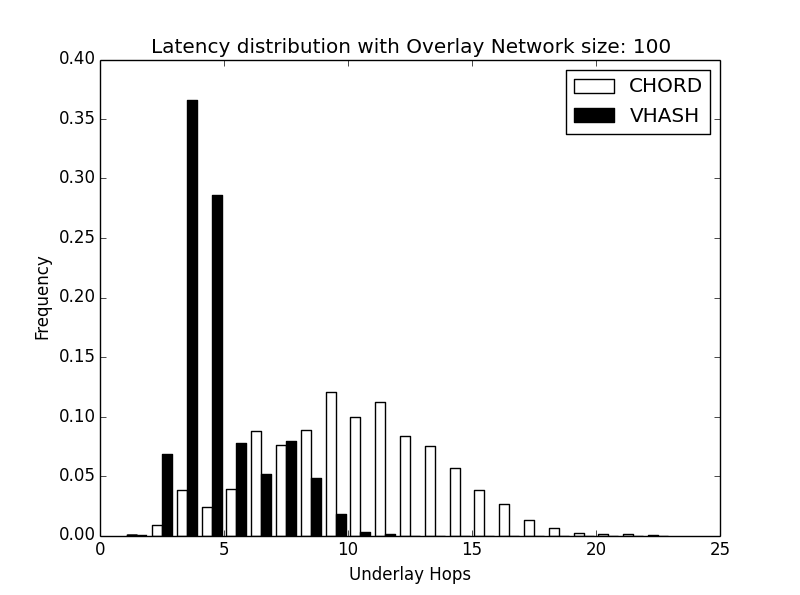
\includegraphics[width=0.5\linewidth]{figs/hist_100}
	\caption{Frequency of path lengths on Chord and VHash in a 100 node overlay.}
	\label{fig:hist100}
\end{subfigure}

\begin{subfigure}{\columnwidth}
	\centering
	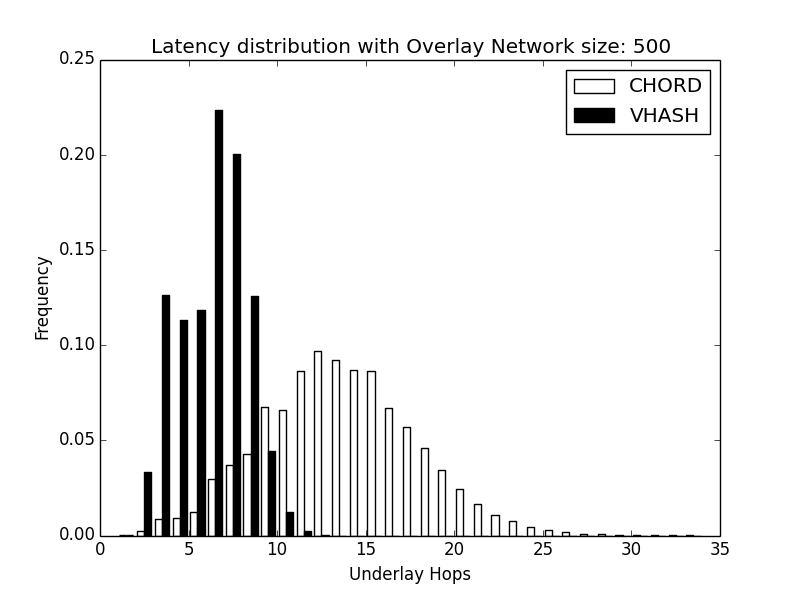
\includegraphics[width=0.5\linewidth]{figs/hist_500}
	\caption{Frequency of path lengths on Chord and VHash in a 500 node overlay.}
	\label{fig:hist500}
\end{subfigure}

\begin{subfigure}{\columnwidth}
	\centering
	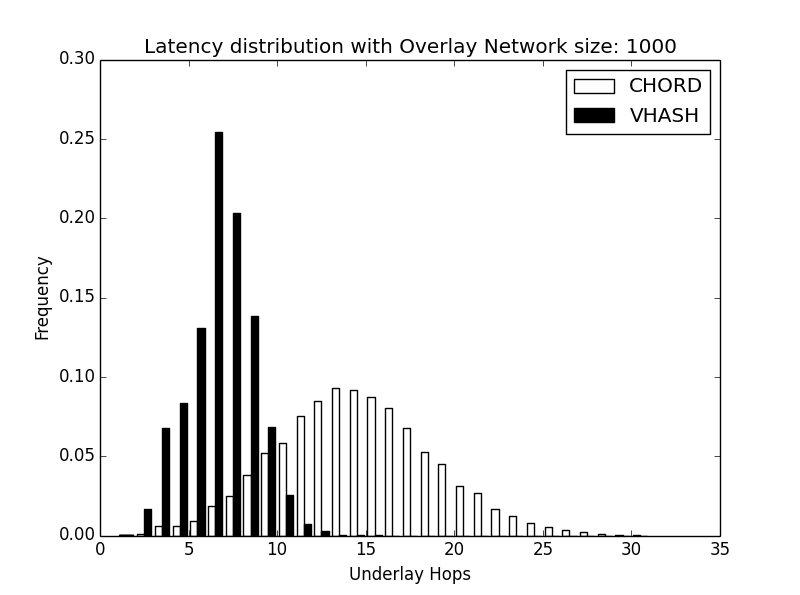
\includegraphics[width=0.5\linewidth]{figs/hist_1000}
	\caption{Frequency of path lengths on Chord and VHash in a 1000 node overlay.}
	\label{fig:hist1000}
\end{subfigure}

\caption{Figures \ref{fig:hist100}, \ref{fig:hist500}, and \ref{fig:hist1000} show the difference in the performance of Chord and VHash for 10,000 routing samples on a 10,000 node underlay network for differently sized overlays.
The Y axis shows the observed frequencies and the X axis shows the number of hops traversed on the underlay network.
VHash consistently requires fewer hops for routing than Chord.}
\label{fig:hist}

\end{figure}




Figure \ref{fig:hist} shows the distribution of path lengths measured in underlay hops in both Chord and VHash.
VHash significantly outperformed Chord and considerably reduced the underlay path lengths in three network sizes.

We also sampled the lookup length measured in overlay hops for a 1000 sized Chord and VHash network.
As seen in Figure \ref{fig:histover}, the paths measured in overlay for VHash were significantly shorter than those in Chord.
In comparing the overlay and underlay hops, we find that for each overlay hop in Chord, the lookup must travel 2.719 underlay hops on average; in VHash, lookups must travel 2.291 underlay hops on average for every overlay hop traversed.

Recall that this work is based on scale free networks, where latency improvements are difficult.
An improvement of 0.4 hops over a diameter of 3 hops is significant.
VHash has on average less overlay hops per lookup than Chord, and for each of these overlay hops we consistently traverse more efficiently across the underlay network.
\begin{figure}
	\centering
	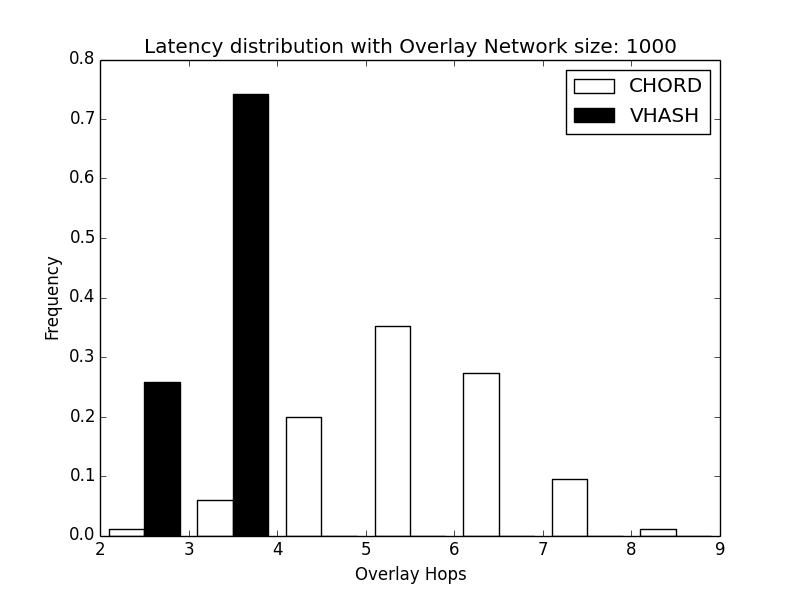
\includegraphics[width=0.5\linewidth]{figs/hist_overlay_4d}
	\caption{Comparison of Chord and VHash in terms of overlay hops.  Each overlay has 1000 nodes.  The Y axis denotes the observed frequencies of overlay hops and the X axis corresponds to the path lengths in overlay hops.}
	\label{fig:histover}
\end{figure}




\subsection{Remarks}

Voronoi tessellations have a wide potential for applications in ad-hoc networks, massively multiplayer games, P2P, and distributed networks.
However, centralized algorithms for Voronoi tessellation and Delaunay triangulation are not applicable to decentralized systems.
In addition, solving Voronoi tessellations in more than 2 dimensions is computationally expensive.

We created a distributed heuristic for Voronoi tessellations in an arbitrary number of dimensions.
Our heuristic is fast and scalable, with a expected memory cost of $(3d+1)^{2}+3d+1$ and expected maximum runtime of O$(\frac{\log^{2} N}{\log^{2} \log N} )$.

We ran two sets of experiments to demonstrate VHash's effectiveness.
Our first set of experiments demonstrated that our heuristic is reasonably accurate  and our second set demonstrates that reasonably accurate is sufficient to build a P2P network which can route accurately.
Our second experiment showed that VHash  could significantly reduced the latency in Distributed Hash Tables.

%Our next step is to create a formal protocol and implementation for a Voronoi tessellation-based distributed hash table using DGVH.
%We can use this DHT to choose certain metrics we want to measure, such as latency, or trust, and embed that information as part of a node's identity.
%By creating an appropriate distance measurement, we can route along some path that minimizes or maximizes the desired metric.
%Rather than create an overlay that minimizes hops, we can have our overlay minimize latency, which is the actual goal of most routing algorithms.

%\subsection*{Peerlist and Topology}
%Like CAN \cite{can}, VHash tracks only neighbors for it's peers.
%We enforce a lower limit on the size of the peerlist to avoid nodes being


%\subsection*{Joining}


%\subsection*{Fault Tolerance}




\section{ChordReduce}
DHTs have received a great deal of research due to their popularity as the backbone for structured P2P system primarily used for file-sharing.
There are two recent and fairly open questions that we want to examine.

\begin{enumerate}
	\item How and in what contexts  can DHTs effectively be used for distributed computations?
	\item How can nodes in a DHT autonomously detect and redistribute imbalances in the network load?
\end{enumerate}

This section will talk about ChordReduce, in which we have made preliminary attempts to answer the first question by implementing MapReduce on a DHT.
The next section, Section \ref{sec:auto-load-bal}, discusses the our preliminary work in answering the second.

\subsection{Background and Motivation}

Distributed computing is a current trend and will continue to be the approach for intensive  applications.
We see this in the development of cloud computing \cite{p2p-cloud}, volunteer computing frameworks like BOINC \cite{anderson2004boinc} and Folding@Home \cite{larson2002folding}, and MapReduce  \cite{mapreduce}.
Google's MapReduce  in particular has rapidly become an integral part in the world of data processing.
A user can use MapReduce to take a large problem, split it into small, equivalent tasks and send those tasks to other processors for computation.
The results are sent back to the user and combined into one answer.

Popular platforms for MapReduce, such as Hadoop \cite{hadoop}  \cite{shvachko2010hadoop}, are explicitly designed to be used in large datacenters \cite{hadoopAssumptions} and the majority of research has been focused there.
However, as we have previously mentioned, there are notable issues with a centralized design.

First and foremost is the issue of fault-tolerance.
Centralized designs have a single point of failure \cite{shvachko2010hadoop}.
So long as all computing resources are located in one geographical area or rely on a particular node, a power outage or catastrophic event could interrupt computations or otherwise disrupt the platform \cite{babaoglu2014people}.

A centralized design assumes that the network is relatively unchanging and may not have mechanisms to handle node failure during execution or, conversely, cannot speed up the execution of a job by adding additional workers on the fly.
Many environments also anticipate a certain degree in homogeneity in the system.
Finally deploying these systems and developing programs for them has an extremely steep learning curve.

There is no reason that these assumptions need to be the case for MapReduce, or for many distributed computing frameworks in general.
Moving away from the data center context opens up more possibilities for distributed computing, such as P2P clouds \cite{p2p-cloud}.
However, without a centralized framework, the network needs some kind of protocol to organize the various components in the network.
As part of our research, we developed a highly robust and distributed MapReduce framework based on Chord, called ChordReduce \cite{chordreduce}.

There a number of reasons to used a DHT as the protocol for a distributed computing platform.
First, nodes ID and their location in the network are strongly bound to what data they are responsible for, such that any node can lookup which node is responsible a particular piece of data.
This obviates the need for a centralized organizer to maintain this bit of metadata or assign backups for data, as nodes can do this autonomously.
DHTs assume that the network is heterogeneous, rather than homogeneous.
They have been used for over a decade for P2P file-sharing applications for these reasons.


%\subsubsection{P2P cloud}
%http://www.cs.unibo.it:443/pub/TR/UBLCS/2011/2011-10.pdf

%Clouds and Volunteer Computing platforms are different.
%Clouds@home
%Nanodatacenter

\subsection{What is ChordReduce?}

ChordReduce \cite{chordreduce} is designed as a more abstract framework for MapReduce, able to run on any arbitrary distributed configuration.
ChordReduce leverages the features of distributed hash tables to handle distributed file storage, fault tolerance, and lookup.
We designed ChordReduce to ensure that no single node is a point of failure and that there is no need for any node to coordinate the efforts of other nodes during processing.

\begin{figure}
	\centering
	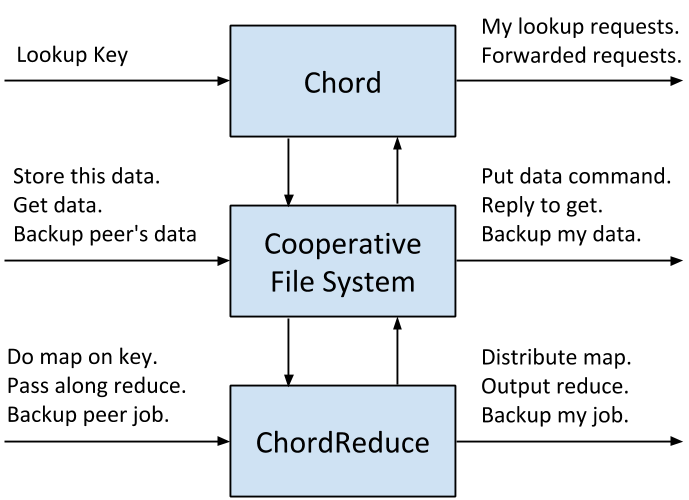
\includegraphics[width=0.8\linewidth]{figs/CR_architecture}
	\caption{A simple architectural diagram of the layers of ChordReduce.}	
	\label{fig:cr_arch}
\end{figure}



\subsubsection{File System}
Our central design philosophy was to leverage as many features of the underlying DHT as possible.
For example, we do not need to create a new distributed file system, as we can just use the DHT to hash file identifiers and use the DHT to store the file at the node responsible for that key.

If the file is large, we can instead use Dabek et al.'s Cooperative File System or CFS \cite{CFS}.
In CFS, files are split into approximately equally sized blocks.
Each block is treated as an individual file and is assigned a key equal to the hash of its contents.
The block is then stored at the node responsible for that key.
The node that would normally be responsible for the whole file instead stores a \textit{keyfile}.
The keyfile is an ordered list of the keys corresponding to the files' block and is created as the blocks are assigned their respective keys.
When the user wants to retrieve a file, they first obtain the keyfile and then request each block specified in the keyfile.


\subsubsection{Computation}
ChordReduce treats each task or target computation as an object of data.
This means we can distribute them in the same manner as files and rely on the protocol to route them and provide robustness.


In ChordReduce, each node takes on responsibilities of both a worker node and master node, in the same way that a node in a P2P file-sharing service acts as both a client and a server.
A user starts a job, contacts a node at a specified hash address and provides it with the tasks.
This address can be chosen arbitrarily or be a known node in the ring.
We call this node the \textit{stager} for this particular job.

The job of the stager is to divide the work into \emph{data atoms}, the smallest units of work.
This might represent a block of text, the result of a summation for a particular intermediate value, or a subset of items to be sorted.
The specifics of how to divide the work are defined by the user in a \emph{stage} function.
The data atoms also contain user created Map and Reduce functions.

If the user wants to perform a MapReduce job on a particular file on the network, the stager locates the keyfile for the data and creates a data atom for each block in the file.
Each data atom is then sent to the node responsible for their corresponding block.
When the data atom reaches its destination node, that node retrieves the necessary data and applies the Map function.
The results are stored in a new data atom,  which are then sent back to the stager's hash address (or some other user defined address).
This will take $O(\lg n)$ hops traveling over Chord's fingers.
At each hop, the node waits a predetermined minimal amount of time to accumulate additional results (In our experiments, this was 100 milliseconds).
Nodes that receive at least two results merge them using the Reduce function.
The results are continually merged until only one remains at the hash address of the stager.


Some MapReduce jobs do not rely on a file stored on the network, such as a Monte-Carlo approximation.
In this situation, the data atoms define a task to be run multiple times.
In this case, the created data atoms are then each given a random hash and sent to the node responsible for that hash address, guaranteeing they are evenly distributed throughout the network.
From there, the execution is identical to the above scenario.


%Once the data atoms are sent out, the stager's job is done and it behaves like any other node in the network. The staging period is the only time ChordReduce is vulnerable to churn, and only if the stager leaves the ring in the middle of sending out data atoms.  The user would get some results back, but only for the data the stager managed to send out.

Once all the Reduce tasks are finished, the user retrieves the results from the node at the stager's address.
This may not be the stager himself, as the stager may no longer be in the network.
The stager does not need to collect the results himself, since the work is sent to the stager's hash address, rather than the stager itself.
Thus, the stager could quit the network after staging, and both the user and the network would be unaffected by the change.
This eliminates the need for a single specific root node and provides fault tolerance.
% Here, we are leverging two features. First, we use the automatic assignment of responsibility to automatically route the data to the sucessor.  %Second, the same process Chord uses to backup files is used to backup the intermediate data.

Similar precautions are taken for nodes working on Map and Reduce tasks.
Those tasks are backed up by a node's successor, who will run the task if the node leaves before finishing its work (e.g. the successor loses his predecessor).
The task is given a timeout by the node.
If the backup node detects that the responsible node has failed, he starts the work and backs up again to \emph{his} successor.
Otherwise, the data is tossed once the timeout expires.
This is done to prevent a job being submitted twice.

An advantage of our system is the ease of development and deployment.
The developer does not need to worry about distributing work evenly, nor does he have to worry about any node in the network going down.
The stager does not need to keep track of the status of the network.
The underlying Chord ring handles that automatically.
If the user finds they need additional processing power during runtime, they can boot up additional nodes, which would automatically be assigned work based on their hash value.
If a node goes down while performing an operation, his successor takes over for him.
This makes the system extremely robust during runtime.


\subsubsection{Robustness}
Since the system is distributed, we need to assume that any member of the network can go down at any time.
When a node fails or leaves Chord, the failed node's successor will become responsible for all of the failed nodes keys.
Likewise, each node in the ChordReduce network relies on their successor to act as a backup.

To prevent data from becoming irretrievable, each node periodically sends backups to its successor.
In order to prevent a cascade of backups of backups, the node only sends data that it is currently responsible for.
This changes as nodes enter and leave the network.
If a node's successor leaves, the node sends a backup to his new successor.
If the node fails, the successor is able to take his place almost immediately.
The backup  scheme is used to not only backup files, but the computational tasks as well.

This procedure prevents any single node failure or sequences of failures from harming the network.
Only the failure of multiple neighboring nodes poses a threat to the network's integrity.
Recall that a node's ID in the network does not map to a geographical locations.
Any failure that affects multiple nodes simultaneously would be spread uniformly throughout the network.
This means if successive nodes to fail simultaneously, they do so independently.

Assume node has failure rate $r < 1$ and that the each node backs up their data with $s$ successive nodes downstream.
If one of these nodes fail, the next successive node takes its place and the next upstream node becomes another backup.
This ensures there will always be $s$ backups.
The integrity of the ring would only be jeopardized if $s+1$ successive nodes failed simultaneously.
The chances of this would be $r^s+1$, as each failure would be independent.


A final consequence of this is load-balancing during runtime.
When a joining node $n$ find his successor, $n$ asks if the successor is holding any data $n$ should be responsible for.
The successor looks at all the data $n$ is responsible for and sends it to $n$.
The successor maintains this data as a backup for $n$.
Because Map tasks are backed up in the same manner as data, a node can take the data and corresponding tasks he is responsible for and begin performing Map tasks immediately.

\subsection{Experiments}

We created a prototype of ChordReduce in order to demonstrate it was a viable framework \cite{chordreduce}.
To acheive this, we had to show ChordReduce had these three properties:
\begin{enumerate}
	\item ChordReduce provided significant speedup during a distributed job.
	\item ChordReduce scaled.
	\item ChordReduce handled churn during execution.
\end{enumerate}


We needed to demonstrate speedup by showing that a job handled by multiple workers generally finished sooner than the same job handled by a single worker.  
More formally we must establish that $\exists n$ such that $T_{n} < T_{1}$, where $T_{n}$ is the amount of time it takes for $n$ nodes to finish the job.

To establish scalability, we had to show that the cost of distributing the work grows logarithmically with the number of workers.  
We needed to demonstrate that the larger the job is, the more nodes can work on the problem before we begin experiencing diminishing returns. 
This can be stated as $$T_{n} = \frac{T_{1}}{n} + k \cdot \log_{2}(n)$$, where $\frac{T_{1}}{n}$ is the amount of time the job would take when distributed in an ideal universe and $k \cdot \log_{2}(n)$ is network induced overhead, $k$ being an unknown constant dependent on network latency and available processing power.

Finally, to demonstrate robustness, we had to show that ChordReduce can handle arbitrary node failure in the ring and that such failures minimally impacted the overall speed of computation

\subsubsection{Setup}


To stress test our framework, we ran a Monte-Carlo approximation of $\pi$. 
This process is analogous to having a square containing  the top-right quadrant of a circle (Figure \ref{fig:dartboard}), and then throwing darts at random locations.  
Counting the ratio of darts that land inside the circle to the total number of throws yields an approximation of $\frac{\pi}{4}$.  
The more darts we throw, i.e. the more samples that are taken, the more accurate the approximation.\footnote{This is not and was not intended to be a particularly good approximation of $\pi$.
Each additional digit of accuracy requires increasing the number of samples taken by an order of magnitude.}


We chose this experiment for a number of reasons. 
The job is extremely easy to distribute.  
This also made it very easy to test scalability. 
By doubling the amount of samples, we can double the amount of work each node gets.  
We could also test the effectiveness of distributing the job among different numbers of workers.


\begin{figure}
	\centering
	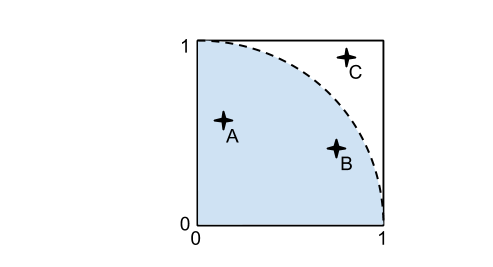
\includegraphics[width=0.5\linewidth]{figs/dartboard}
	\caption{The "dartboard." The computer throws a dart by choosing a random $x$ and $y$ between 0 and 1.  If $x^{2} + y^{2} < 1^{2} $, the dart landed inside the circle.  $A$ and $B$ are darts that landed inside the circle, while $C$ did not.}
	\label{fig:dartboard}
\end{figure}


Each Map job was defined as the number of throws the node must make and yielded total number of throws and the number of throws that landed inside the circular section.  
Reducing these results was then a matter of adding the respective fields together. 

We ran our experiments using Amazons's Elastic Compute Cloud (EC2) service.  
Amazon EC2 allows users to purchase an arbitrary amount of virtual machines by the hour. 
Each node was an individual EC2 small instance with a preconfigured Ubuntu 12.04 image.  
%These instances were capable enough to provide constant computation, but still weak enough that they would be overwhelmed by traffic on occasions, creating a constant churn effect in the ring.  

Once started, nodes retrieved the latest version of the code and run it as a service, automatically joining the network.  
We could choose any arbitrary node as the stager and tell it to run the MapReduce process. 
We found that the network was robust enough that we could take a node we wanted to be the stager out of the network, modify its MapReduce test code, have it rejoin the network, and then run the new code without any problems. 
Since only the stager had to know how to create the Map tasks, the other nodes did not have to be updated and execute the new tasks they are given.

We ran our experiments on groups of 1, 10, 20, 30, and 40 workers, which generated a $10^{8}$ sample set and a $10^{9}$ sample set.
Additionally, we gathered data on a $10^{7}$ sample set using 1, 5, 10, 20, 30 workers.  
To test churn, we ran an experiment where each node had an equal chance of leaving and joining the network and varied the level of churn over multiple runs.  

We also utilized a subroutine we wrote called $plot$, which sends a message sequentially around the ring to establish how many members there are.  
If $plot$ failed to return in under a second, the ring was experiencing structural instability.

\begin{figure}
	\centering
	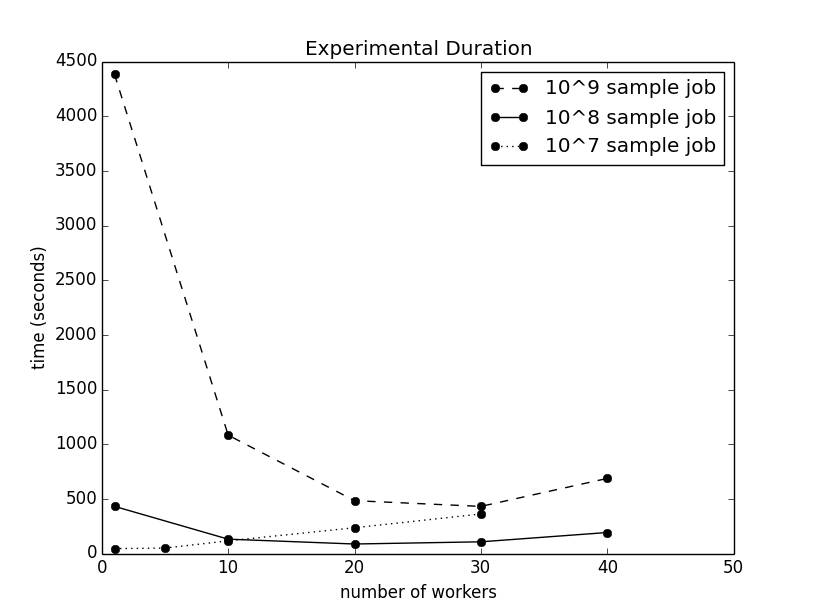
\includegraphics[width=0.5\linewidth]{figs/expTime}
	\caption{Our results show that for a sufficiently large job, it was almost always preferable to distribute it.  
		When the job is too small, such as with the $10^{7}$ data set, our runtime is dominated by the overhead.  
		Our results are what we would expect when overhead grows logarithmically to the number of workers.}
	\label{fig:expTime}
\end{figure}


\begin{figure}
	\centering
	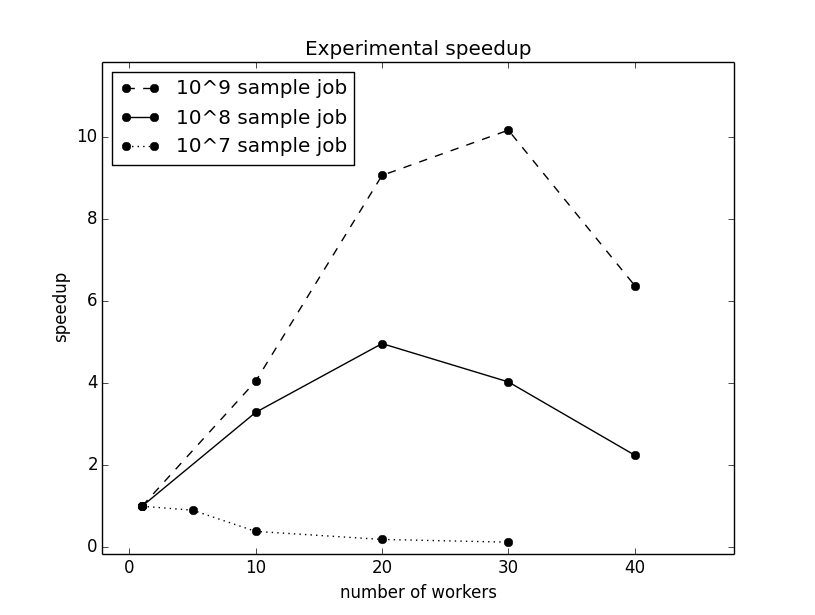
\includegraphics[width=0.5\linewidth]{figs/expSpeed}
	\caption{The larger the size of the job, the greater the gains of distributing with ChordReduce.  In addition, the larger the job, the more workers can be added before we start seeing diminishing returns.  This demonstrates that ChordReduce is scalable.}
	\label{fig:expSpeed}
\end{figure}

Figure \ref{fig:expTime} and Figure \ref{fig:expSpeed} summarize the experimental results of job duration and speedup.  
Our default series was the $10^{8}$ samples series.  
On average, it took a single node 431 seconds, or approximately 7 minutes, to generate $10^{8}$ samples.  
Generating the same number of samples using ChordReduce over 10, 20, 30, or 40 nodes was always quicker.  
The samples were generated fastest when there were 20 workers, with a speedup factor of 4.96, while increasing the number of workers to 30 yielded a speedup of only 4.03.  
At 30 nodes, the gains of distributing the work were present, but the cost of overhead ($k \cdot \log_{2}(n)$) had more of an impact.  
This effect is more pronounced at 40 workers, which experienced  a speedup of only 2.25.

Since our data showed that approximating $\pi$ on one node with $10^{8}$ samples took approximately 7 minutes, collecting $10^{9}$ samples on a single node would take 70 minutes at minimum.  
Figure \ref{fig:expSpeed} shows that the $10^{9}$ set gained greater benefit from being distributed than the $10^{8}$ set, with the speedup factor at 20 workers being 9.07 compared to 4.03.  
In addition, dimishing returns only showed up at 40 workers, compared with the $10^{8}$ data set, which began its drop off at 30 workers.
This behavior showed that the larger the job being distributed, the greater the gains of distributing the work using ChordReduce.

The $10^{7}$ sample set confirms that the network overhead is logarithmic.  
At that size, it is not effective to run the job concurrently and we start seeing overheard acting as the dominant factor in runtime.  
This matches the behavior predicted by our equation, $T_{n} = \frac{T_{1}}{n} + k \cdot \log_{2}(n)$. 
For a small $T_{1}$, $\frac{T_{1}}{n}$  approaches 0 as $n$ gets larger, while $k \cdot \log_{2}(n)$, our overhead, dominates the sample.  
The samples from our data set fit this behavior, establishing that our overhead increases logarithmically with the number of workers.


\begin{figure}
	\centering
	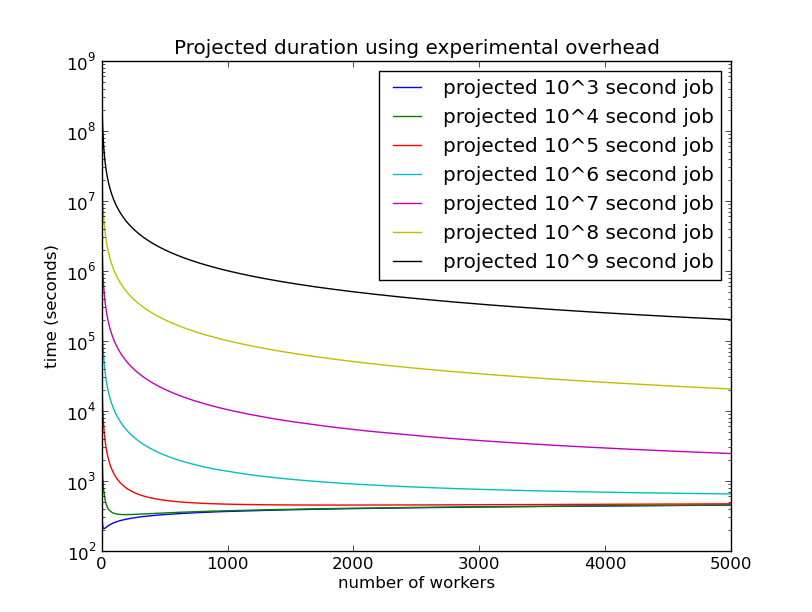
\includegraphics[width=0.5\linewidth]{figs/projTime}
	\caption{The projected runtime using ChordReduce for differently sized jobs.  Each curve projects the expected behavior for job that takes a single worker the specified amount of time.}
	\label{fig:projTime}
\end{figure}

\begin{figure}
	\centering
	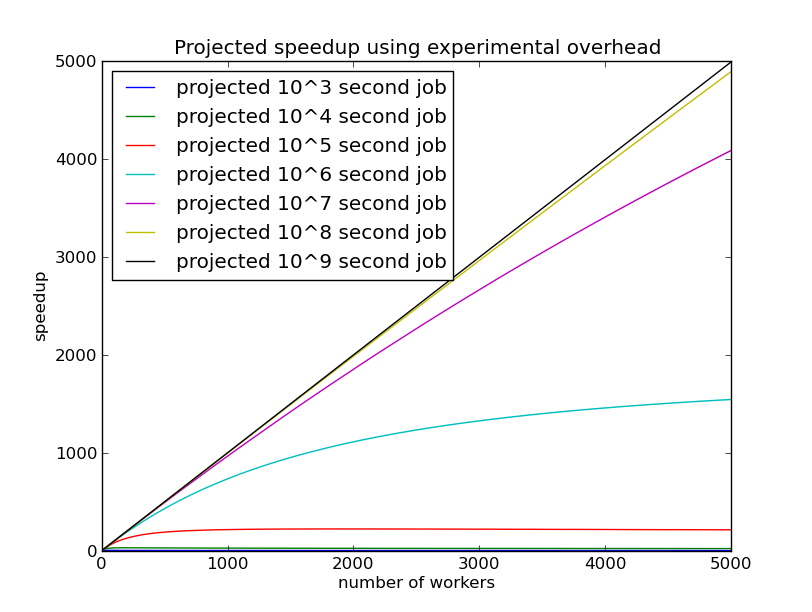
\includegraphics[width=0.5\linewidth]{figs/projSpeed}
	\caption{The projected speedup for different sized jobs. }
	\label{fig:projSpeed}
\end{figure}

Since we were able to establish that $T_{n} = \frac{T_{1}}{n} + k \cdot \log_{2}(n)$, we created an estimate how long a job that takes an arbitrary amount of time to run on a single node would take using ChordReduce.  
Our data points indicated that the mean value of $k$ for this problem was 36.5.  
Figure \ref{fig:projTime} shows that any jobs that would take more than $10^{4}$ seconds for single worker, we can expect there would still be benefit to adding an additional worker, even when there are already 5000 workers already in the ring.  
Figure \ref{fig:projSpeed} further emphasizes this. Note that as the jobs become larger, the expected speedup from ChordReduce  approaches linear behavior.


Table \ref{tab:churnSpeed} shows the experimental results for different rates of churn. 
We discus these experimental results and their significance in Section \ref{sec:auto-load-bal}.
\begin{table}
	\centering
	\begin{tabular}{|r|r|r|}
		\hline
		Churn rate per second & Average runtime (s) & Speedup vs 0\% churn\\ \hline{}
		0.8\% & 191.25 & 2.15 \\ \hline
		0.4\% & 329.20 & 1.25 \\ \hline
		0.025\% & 431.86 & 0.95 \\ \hline
		0.00775\%  & 445.47 & 0.92 \\ \hline
		0.00250\% & 331.80  &  1.24 \\ \hline
		0\% & 441.57 & 1.00 \\ \hline
	\end{tabular}
	\caption{}
	\label{tab:churnSpeed}
\end{table}


%These results show the system  is relatively insensitive to churn.  
%We started with 40 nodes in the ring and generated $10^{8}$ samples while experiencing different rates of churn, as specified in Table \ref{churnSpeed}.  
%At the 0.8\% rate of churn, there is a 0.8\% chance each second that any given node will leave the network followed by another node joining the network at a different location. 
%The joining rate and leaving rate being identical is not an unusual assumption to make \cite{marozzo2012p2p} \cite{load}.

%Our testing rates for churn are an order of magnitude higher than the rates used in the P2P-MapReduce simulation  \cite{marozzo2012p2p}.  In their paper, the highest rate of churn was only 0.4\% per minute. Because we were dealing with fewer nodes, we chose larger rates to demonstrate that ChordReduce could effectively handle a high level of churn.


Our experiments show that for a given problem, ChordReduce can effectively distribute the problem, yielding a substantial speedup.  
Furthermore, our results showed that the larger the problem is, the more workers could be added before diminishing returns were incurred.  
During runtime, we experienced multiple instances where $plot$ would fail to run and the stager would report socket errors, indicating that it had lost connection with a node in the ring.  Despite this turbulence, every node managed to reestablish connection with each other and report back all the data.  
This further demonstrated that we were able to handle the churn in the network.


\subsection{Heterogeneity Calculation}

One of the advantages to using homogeneous hardware is that each machine, each core, each node is the same.
To evenly distribute the workload, you just have to give each machine the same amount of work.
While a

This is more difficult in a heterogeneous system, such as ChordReduce, as each machine can shoulder a different amount of work.
How do we distribute work evenly across a heterogeneous system?

We can solve this by adjusting the amount of nodes representing each machine in the network.
Machines that can handle a larger load create more nodes in the network.
Besides solving the heterogeneous load-balancing problem, increasing the number of nodes in the system increases the overall load-balancing of the system.

The question we must answer is ``how?''
We need to create some unit of measurement for a distributed computing system and research if any other researchers have asked this problem.
Furthermore, this measurement might need to be relative to other nodes in the network, since the only basis for comparison are the scores of the peers. 
Finally, this process needs to be handled autonomously by each node.
This is part of the proposed work discussed in Chapter \ref{chapter:experiments}.
\section{Autonomous Load Balancing}
\label{sec:auto-load-bal}


During our experiments testing the capabilities of ChordReduce, we experienced a significant and completely unexpected anomaly while testing churn.
One of the things previous research \cite{marozzo2012p2p}  \cite{leemap} in the same area we felt we needed to explore better was how a completely decentralized computation could handle churn.
Now, despite our initial prototype having numerous bugs and only able to handle small networks, we were fairly certain of it's ability to handle churn.

Marozzo et al.\ \cite{marozzo2012p2p} tested their network using churn rates of 0.025\%, 0.05\%, 0.1\%, 0.2\%, and 0.4\% per minute.
The churn rate of $cr << 1$ per minute means that each minute on average, $cr \cdot n$ nodes leave the network and $cr \cdot n$  new nodes join the network.\footnote{It is standard practice to assume the joining rate and leaving rate are equal.}
This could effectively be thought of as each node flipping a weighted coin every minute.
When the coin lands on tails, the node leaves.
A similar process happens for nodes wanting to join the network.

We wanted the robustness of our system to be beyond reproach, so we tested at rates from 0.0025\% to 0.8\% \textbf{\textit{per second}}, 120 times the fastest rate used to test P2P-MapReduce.
This is an absurdly fast and unrealistic speed, the only purpose of which was to cement the fault tolerance of the system.
Since we were testing ChordReduce on Amazon's EC2 and paying per instance per hour, we limited the number of nodes.
Rather than having a pool of nodes waiting to join the network, we conserved our funds by having leaving nodes immediately rejoin the network under a new IP/port combo.
The meant our churn operation was essentially a simultaneous leave and join.


What we found was that jobs on ChordReduce finished twice as fast under the unrealistic levels churn (0.8\% per second) than no churn (Table \ref{tab:churnSpeed}).
This completely mystified us.
Churn is a disruptive force; how can it be aiding the network?

\subsection*{Hypothesis}
We hypothesize this was due to the number of data pieces (larger) vs the number of workers (smaller).
There were more workers than there were pieces of data, so some workers ended up with more data than others in the initial distribution.
This means that there was some imbalance in the way data was distributed among nodes.
This was \textit{further} exacerbated by small number of workers distributed over a large hash space, leading some nodes to have larger swaths of responsibility than others.

Given this setup, without any churn, the operation would be:
Workers get triggered, they start working, and the ones with little work finish their work quickly, and the network waits for the node with higher loads of work.

Its important to note here that the work in ChordReduce was performed atomically, a piece at a time.
When a node was working on a piece, it informed it's successor, then informed them when it finished.
These pieces of work were also small, possibly too small.

As mentioned previously, under our induced experimental churn, we had the nodes randomly fail and immediately join under a new IP/port combination, which yields a new hash.
The failure rates were orders of magnitude higher than what would be expected in a ``real'' (nonexperimental) environment.
The following possibilities could occur:
\begin{itemize}
	\item A node without any active jobs leaves.
	It dies and and comes back with a new port chosen.
	This new ID has a higher chance of landing in a larger region of responsibility (since new joining nodes have a greater chance of hashing to a larger region than a smaller).
	In other words, it has a (relatively) higher chance of moving into an space where it becomes acquires responsibility for enqueued jobs.
	The outcomes of this are:
	\begin{itemize}
		\item The node rejoins in a region and does not acquire any new jobs.
		This has no impact on the network (Case I).
		\item The node rejoins in a region that has jobs waiting to be done.
		It acquires some of these jobs.
		This speeds up performance (Case II).
	\end{itemize}
	\item A node with active jobs dies.
	It rejoins in a new space.
	The jobs were small, so not too much time is lost on the active job, and the enqueued jobs are backed up and the successor knows to complete them.
	However, the node can rejoin in a more job-heavy region and acquire new jobs.
	The outcomes of this are:
	\begin{itemize}
		\item A minor negative impact on runtime and load balancing (since the successor has more jobs to handle) (Case III).
		\item A possible counterbalance in load balancing by acquiring new jobs off a busy node (Case IV).
	\end{itemize}
\end{itemize}

The longer the nodes work on the jobs, the more nodes finish and have no jobs.
This means as time increases, so do the occurrences of Case I and II.


This leads us to two hypotheses:
\begin{itemize}
	\item Deleting nodes motivates other nodes to work harder to avoid deletion (a ``beatings will continue until morale improves'' situation).
	\item Our high rate of churn was dynamically load-balancing the network.
	It appears even the smallest effort of trying to dynamically load balance, such as rebooting random nodes to new locations, has benefits for runtime.
	Our method is a poor approximation of dynamic load-balancing, and it still shows improvement.
\end{itemize}

The first hypothesis is mentally pleasing to anyone who has tried to create a distributed system, but lacks rigor.
We still have to verify the existence of this phenomena in an independent experiment, and establish that it does is part of the proposed work (Chapter \ref{chapter:experiments}).


Once we have established that it does exist, we need a better load-balancing strategy than randomly inducing.
We want nodes to have a precomputed list of locations in which they can insert nodes to perform load-balancing on an ad-hoc basis during runtime.
This precomputed list ties directly into the security research on DHTs we have done \cite{sybil-analysis}.


%The questions and goals here are straightforward:
%\begin{itemize}
%	\item Further establish the phenomena exists.
%	\item We stumbled across this phenomena with a brute force method and still got promising results.
%	Can we create a more accurate and mean
%	\item Can this phenomena be stochastically modeled or otherwise predicted via theoretical analysis?
%	\item In what contexts can this be used for DHTs?  Distributed computing?  Replication for file sharing?

%\end{itemize}






\section{Sybil Attacks and Injection}
One of the key properties of structured peer-to-peer (P2P) systems is the lack of a centralized coordinator or authority.
P2P systems remove the vulnerability of a single point of failure and the susceptibility to a denial of service attack \cite{sybil}, but in doing so, open themselves up to new attacks.

Completely decentralized P2P systems are vulnerable to \textit{Eclipse attacks}, whereby an attacker completely occludes healthy nodes from one another.
This prevents them from communicating without being intercepted by the adversary.
Once an Eclipse attack has taken place, the adversary can launch a variety of crippling attacks, such as incorrectly routing messages or returning malicious data \cite{srivatsa2004vulnerabilities}.

One way to accomplish this attack is to perform a \emph{Sybil attack} \cite{sybil}.
In a Sybil attack, the attacker masquerades as multiple nodes, effectively over-representing the attacker's presence in the network to maximize the number of links that can be established with healthy nodes.
If enough malicious nodes are injected into the system, the majority of the nodes will be occluded from one another, successfully performing an Eclipse attack.

%We discovered injecting replicas is easy and simple in P2P networks, we use a Sybil attack.
%This was the focus of my Data Security project
%I hypothesize we can Sybil attacks for improving load balancing on demand.

This vulnerability is well known \cite{dhtsec}.
Extensive research has been done assessing the damage an attacker can do after establishing themselves \cite{srivatsa2004vulnerabilities}.
%Especially when a hash value to assign neighbors
Little focus has been done on examining how the attacker can establish himself in the first place and precisely how easily the Sybil attack can be accomplished.

We did a project that focused on looking at the computational and memory costs of performing the Sybil attack.
The computation costs turn out to be fairly trivial and can be precomputed based on how IDs are assigned, a process we named \textit{mashing}.
If a node obtains their ID via an IP/Port combination, and we limit an attacker to using only ephemeral IP addresses (16383 total), the per node cost of mashing is quite low.
Per node, it takes 48 milliseconds to mash 16383 IP/Port combinations and only 352 kilobytes to store this information after precomputing it.

An attacker would do this for each of his nodes, then join the network and insert as many Sybils as possible.
We calculated that it would take only 1221 IP addresses to compromise 50\% of the links in a 20,000,000 node network \cite{sybil-analysis}.


\subsection{Experiments}
The primary experiment of our project was simulating the complete eclipse a network using a Sybil attack, starting with a single malicious node \cite{sybil-analysis}.
We simulated a network of $n$ nodes, each represented by an ID generated by SHA1 of a random IP/port combination.

The goal of the attacker was to mash as many pairs of adjacent nodes as possible.
We call this the \textit{Nearest Neighbor Eclipse} since the attacker seeks to become the nearest neighbors of each node.

The attacker was given $num\_ips$ randomly generated IP addresses, but could use any port between 49152 and 65535.
This means attacker had $ 16383 \cdot num\_ips $ Sybils at his disposal.
Each of these addresses could  be precomputed by the attacker and stored in a sorted list, requiring only 352 kilobytes per IP.

The adversary in this attack chooses any random hash key as a starting point to ``join'' the network.
This is their first Sybil and the join process provides information about a number of other nodes.
Most importantly, nodes provide information about other nodes that are close to it.
The adversary uses this information to inject Sybils in between successive healthy nodes.
For example, in Pastry, a joining node typically learns about the 16 nodes closest to it for fault tolerance, in addition to all the other nodes it learns about  \cite{pastry}.
In Chord, this number is a system configuration value $r$ \cite{chord}.

We simulated this attack on networks of up to 20 million nodes.
We chose 20 million since it falls neatly into the 15-27 million user range seen on Mainline DHT \cite{mainlineMeasure}.
We gave the attacker access to up to 19 IP addresses.
Our results are in Figures \ref{fig:exp2} and \ref{fig:size_prob_all}.

\begin{figure}
	\centering
	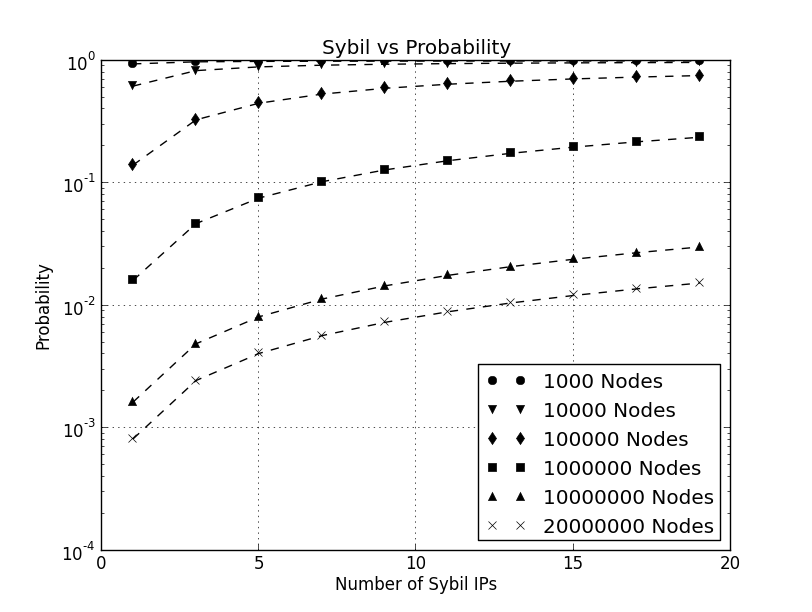
\includegraphics[width=0.5\linewidth]{figs/ip_prob_all}
	\caption[foo]{Our simulation results.  
		The $x$-axis corresponds to the number of IP addresses the adversary can bring to bear.
		The $y$-axis is the probability that any chosen region has been mashed.
		Each line maps to a different network size of $n$.
		The dashed line corresponds to values  $ P_{bad\_neighbor} =  \frac{num\_ips \cdot 16383}{num\_ips \cdot 16383 + n - 1}$, which is the probability a node has a malicious neighbor}
	\label{fig:exp2}
\end{figure}


\begin{figure}
	\centering
	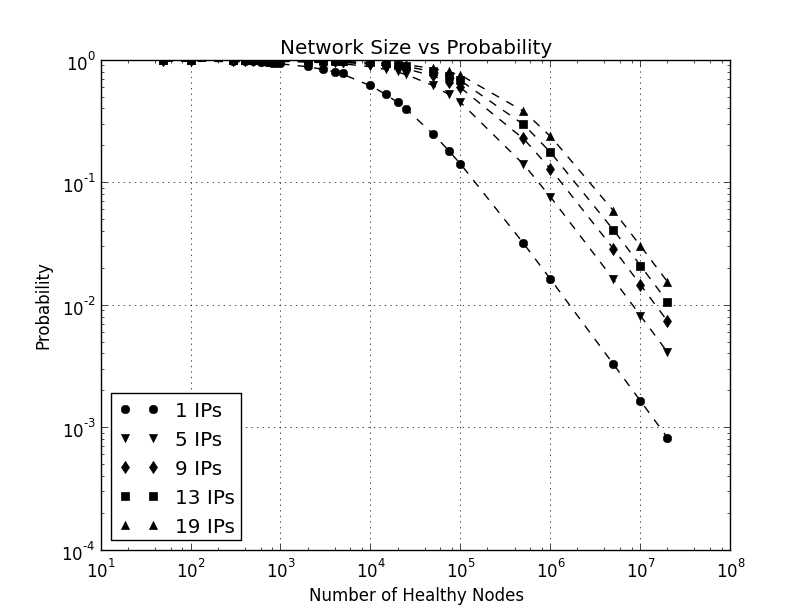
\includegraphics[width=0.5\linewidth]{figs/size_prob_all}
	\caption[a]{These are the same as results shown in Figure \ref{fig:exp2}, but our $x$-axis is the network size $n$ in this case.  
		Here, each line corresponds to a different number of unique IP addresses the adversary has at their disposal.}
	\label{fig:size_prob_all}
\end{figure}


Our results show that an adversary, given only modest resources, can inject a Sybil in between the vast majority of successive nodes in moderately sized networks.
In a large network, modest resources still can be used to compromise more that a third of the network, an  important goal if the adversary  wishes to launch a Byzantine attack.

\subsection{Ramifications}
Our analysis and experiments show that an adversary with limited resources can easily compromise a P2P system and occlude the majority of the paths between nodes.
We can turn this attack around and use to benefit a DHT.
Some nodes will be responsible for larger regions than others and therefore will be responsible for a larger portion of the data.
If a node can detect when a peer is overloaded, the node can inject a virtual node into the region to shoulder some of the load.
The load could be defined by the size of the region or by the volume of traffic.

A network implementing this load-balancing strategy would be self-adaptive.
Nodes in this type of self-adaptive network would have a limited number of virtual nodes to mash.
This limit would protect nodes from becoming overloaded themselves and ensure network stability.
We discuss this further in Chapter \ref{chapter:experiments}.

\section{Summary}
Our previous work has focused primarily on various aspects of Distribute Hash Tables.
We can categorize our research into three distinct, but connected parts:
\begin{description}
	\item[Generalizing DHTs] We developed VHash, which uses the relation between Voronoi tessellation and DHTs to create a more abstract representation of how a DHT operates.
	Using this abstraction, we can embed certain properties into the DHT's topology and optimize these qualities.
	\item[Distributed Computing on a DHT] ChordReduce demonstrated how we can use a DHT to perform MapReduce in a completely decentralized and fault-tolerant environment.
	\item[Autonomous Load Balancing] We have shown that churn had a paradoxically beneficial effect on distributed computations.
	We postulated that we can use this effect to create a more intelligent mechanism for performing autonomous load-balancing, in part based off  the same techniques used to perform a Sybil attack.
	 
\end{description}
It is each of these three parts we wish to further research.
	%\chapter{UrDHT}
\label{chapter:urdht}
%\begin{abstract}
As we have previously discussed, Distributed Hash Tables (DHTs) have an inherent set of qualities, such as greedy routing, maintaining lists of peers which define the topology, and forming an overlay network.
All DHTs use functionally similar protocols to perform lookup, storage, and retrieval operations.
Despite this, no one has created a cohesive formal DHT specification.

Our primary motivation for this project was to create an abstracted model for Distributed Hash Tables based on observations we made during previous research \cite{dgvh}.
We found that all DHTs can cleanly be mapped to the primal-dual problems of Voronoi Tessellation and Delaunay Triangulation.
Rather than having a developer be concerned with the details of a given DHT, we have constructed a new framework, UrDHT, that generalizes the functionality and implementation of various DHTs.

UrDHT is an abstract model of a Distributed Hash Table that implements a self-organizing web of computational units.
It maps the topologies of DHTs to the primal-dual problem of Voronoi Tessellation and Delaunay Triangulation.
By completing a few simple functions, a developer can implement the topology of any DHT in any arbitrary space using UrDHT.
For example, we implemented a DHT operating in a hyperbolic geometry, a previously unexplored nontrivial metric space with potential applications, such as latency embedding.

%Latency embedding will not be included in this paper
%One topology of particular interest we created is a DHT operating within a Poincar\'{e} disk model.
%This DHT could have latency embedded within the overlay and be capable of responding to changes in latency.
%The consequence of this is that, unlike other DHTs, the routing algorithm always uses the shortest latency path to a given destination.

	
%\end{abstract}

%\section{Introduction}
%%Distributed Hash Tables (DHT) have been extensively researched for the past decade.
%Many different DHT protocols have developed over the years.
%What is a DHT
% Mention the DHT API
%Despite this, no one has created a cohesive formal specification for building a DHT. % or something


%UrDHT is our specification and implementation of an abstract DHT.

%
%
%%We present UrDHT, an abstract model of a distributed hash table (DHT). %that solves a number of problems.
%%It is a unified and cohesive model for creating DHTs and P2P applications based on DHTs.
%%%UrDHT also provides a single network for bootstrapping distributed applications.
%%%Third, we show that using the abstraction features of UrDHT, we can embed latency into the DHT's overlay.
%%%
%%%\subsubsection{Abstraction}
%
%Distributed Hash Tables have been the catalyst for the creation of many P2P applications.
%Among these are Redis \cite{redis}, Freenet \cite{freenet}, and, most notably, BitTorrent \cite{bittorrent}. 
%
%
%%TODO Match vocabulary
%UrDHT builds its topology directly upon this insight.
%It uses a greedy distributed heuristic for approximating Delaunay Triangulations.
%We found that we could reproduce the topology of different DHTs by defining a selection heuristic and rejection algorithm for the geometry the DHT.
%For every DHT we implemented, our greedy approximation of Delaunay Triangulation produced a stable DHT, regardless of the geometry.  
%This works in non-Euclidean geometries such as XOR (Kademlia) or even a hyperbolic geometry represented by a Poincar\`{e} disc.
%
%The end result is not only do we have an abstract model of DHTs, we have a simple framework that developers can use to quickly create new distributed applications.
%This simple framework allows generation of internally consistent implementations of different DHTs that can have their performance rigorously compared.  %we can now test DHTs against each other fairly



%\subsubsection{Bootstrapping}
%Another poorly addressed issue within DHTs and DHT-based P2P applications we wish to tackle with UrDHT is the what we have termed the \textit{bootstrapping problem}.
%Simply put, a node can only join the network if it knows another node that is already a member of the network it is trying to join.
%%Current distributed systems suffer from fragmentation, high overhead, and an inability to scale due to difficulty of adoption.
%
%The way this generally works is by having a potential user manually look up at a centralized source, such as the project or application's website, the bootstrapping information for the network.
%It is a philosophical conflict requiring a distributed application to use a centralized source of information to build a distributed network.
%
%UrDHT has the potential to be a distributed source for bootstrapping information for other distributed networks.
%This would make new distributed applications easier to adopt by creating a network to bootstrap \textit{other networks}.
%UrDHT does this by making it easy to add other networks as a service.

%%\subsubsection*{Accomplishments}
%To summarize our contributions:
%\begin{itemize}
%	\item We give a formal specification for what needs to be defined in order to create a functioning DHT.
%	While there has long existed a well known protocol shared by distributed hash tables, this defines what a DHT does.
%	It does not describe what a DHT is.
%	
%	We show that DHTs cleanly map to the primal-dual problem of Delaunay Triangulation and Voronoi Tessellation.
%	We list a set of simple functions that, once defined, allow our Distributed Greedy Voronoi Heuristic (DGVH) to be run in any space, creating a DHT overlay for that space (Section \ref{sec:define}).
%	
%	\item We present UrDHT as an abstract DHT and show how a developer would modify the functions we defined to create an arbitrary new DHT topology (Section \ref{sec:urdht}).
%	
%	\item We show how to reproduce the topology of Chord and Kademlia using UrDHT.
%	We also implement a DHT in a Euclidean geometry and a hyperbolic geometry represented by a Poincar\`{e} disc (Section \ref{sec:implement}).
%%	We also discuss how we can use UrDHT to run subnetworks as a service.
%	\item We conduct experiments that show building DHTs using UrDHT produced efficiently routable networks, regardless of the underlying geometry(Section \ref{sec:experiments}). 
%	\item We present some efforts and projects that are similar to our own (Section \ref{sec:related}).
%	\item We discuss the ramifications of our work and what future work is available (Section \ref{sec:future}).
%\end{itemize}


\section{What Defines a DHT}
\label{sec:define}

A distributed hash table is usually defined by its protocol; in other words, what it can do.
Nodes and data in a DHT are assigned unique\footnote{Unique with astronomically high probability, given a large enough consistent hashing algorithm.} keys via a consistent hashing algorithm.
To make it easier to intuitively understand the context, we will call the key associated with a node its ID and refer to nodes and their IDs interchangeably.

A DHT can perform the \texttt{lookup(key)}, \texttt{get(key)}, and \texttt{store(key, value)} operations.\footnote{There is typically a \textit{delete(key)} operation too, but it is not strictly necessary.}
The \texttt{lookup} operation returns the node responsible for a queried key.
The \texttt{store} function stores that key/value pair in the DHT, while \texttt{get} returns the value associated with that key.

However, these operations define the functionality of a DHT, but do not define the requirements for implementation.
We define the necessary components that comprise DHTs.
We show that these components are essentially Voronoi Tessellation and Delaunay Triangulation.

\subsection{DHTs, Delaunay Triangulation, and Voronoi Tessellation}

Nodes in different DHTs have, what appears at the first glance, wildly disparate ways of keeping track of peers - the other nodes in the network.
However, peers can be split into two groups.

The first group is the \textit{short peers}.
These are the closest peers to the node and define the range of keys the node is responsible for. 
A node is responsible for a key if and only if its ID is closest to the given key in the geometry of the DHT.
Short peers define the DHTs topology and guarantee that the greedy routing algorithm shared by all DHTs works.


%All other peers comprise the \textit{long peers}.
Long peers are the nodes that allow a DHT to achieve faster routing speeds than the topology would allow using only short peers.
This is typically $ O(\log(n)) $ hops, although polylogarithmic time is acceptable \cite{kleinberg2000small}.
A DHT can still function without long peers.

Interestingly, despite the diversity of DHT topologies and how each DHT organizes short and long peers,  all DHTs use functionally identical greedy routing algorithms (Algorithm \ref{alg:routing}):

\begin{algorithm}
	\caption{The DHT Generic Routing algorithm}
	\label{alg:routing}
	%\algsetup{linenosize=\tiny}
	\small
	\begin{algorithmic}[1]
%		\State Given node $n$ and a message being sent to $key$
		\Function{ $n.$lookup}{$(key)$}
			\If{$key \in n$'s range of responsibility}
				\State \Return $ n $
			\EndIf
			\If{ One of $n$'s short peers is responsible for $key$}
				\State \Return the responsible node
			\EndIf
			\State $ candidates $ = $ short\_peers $ + $ long\_peers $
			\State $ next  \leftarrow $  $\min (n$.distance($candidates$, $ key ))$
			\State \Return $next.$lookup($key$)
		\EndFunction
	\end{algorithmic}
	
	\scriptsize
\end{algorithm}
The algorithm is as follows:
If I, the node, am responsible for the key, I return myself.
Otherwise, if I know who is responsible for this key, I return that node.
Finally, if that is not the case, I forward this query to the node I know with shortest distance from the node to the desired key.\footnote{This order matters, as some DHTs such as Chord are unidirectional.} 

Depending of the specific DHT, this algorithm might be implemented either recursively or iteratively.
It will certainly have differences in how a node handles errors, such as how to handle connecting to a node that no longer exists.
This algorithm may possibly be run in parallel, such as in Kademlia \cite{kademlia}.
The base greedy algorithm is always the same regardless of the implementation.


\begin{figure}
	\centering
	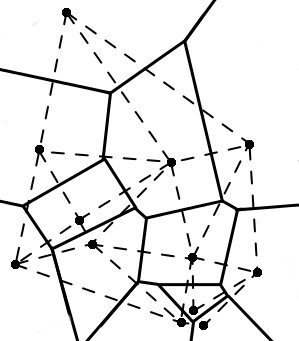
\includegraphics[width=0.75\linewidth]{figs/voronoi}
	\caption{An example Voronoi diagram for objects on a 2-dimensional space.  The black lines correspond to the borders of the Voronoi region, while the dashed lines correspond to the edges of the Delaunay Triangulation.}
	\label{fig:voro-ex}
\end{figure}


With the components of a DHT defined above, we can now show the relationship between DHTs and the primal-dual problems of Delaunay Triangulation and Voronoi Tessellation.
An example Delaunay Triangulation and Voronoi Tessellation is show in Figure \ref{fig:voro-ex}.

%TODO A one-dimensional voronoi fig as example
We can map a given node's ID to a point in a space and the set of short peers to the Delaunay Triangulation.
This would make the range of keys a node is responsible correspond to the node's Voronoi region.
Long peers serve as shortcuts across the mesh formed by Delaunay Triangulation.


Thus, if we can calculate the Delaunay Triangulation between nodes in a DHT, we have a generalized means of creating the overlay network.
This can be done with any algorithm that calculates the Delaunay Triangulation.

Computing the Delaunay Triangulation and/or the Voronoi Tessellation of a set of points is a well analyzed problem.
Many algorithms exist which efficiently compute a Voronoi Tessellation for a given set of points on a plane, such as Fortune's sweep line algorithm \cite{fortune1987sweepline}.

However, DHTs are completed decentralized, with no single node having global knowledge of the topology.
Many of the algorithms to compute Delaunay Triangulation and/or Voronoi Tessellation are unsuited to a distributed environment.
In addition, the computational cost increases when we move into spaces with greater than two dimensions.
In general, finding the Delaunay Triangulation of $n$ points in a space with $d$ dimensions takes $O(n^{\frac{2d-1}{d}})$ time \cite{watson1981computing}.


Is there an algorithm we can use to efficiently calculate Delaunay Triangulation for a distributed system in an arbitrary space?
We created an algorithm called the Distributed Greedy Voronoi Heuristic (DGVH), explained below \cite{dgvh}.


\subsection{Distributed Greedy Voronoi Heuristic}
\label{sec:dgvh}


The Distributed Greedy Voronoi Heuristic (DGVH) is an efficient method for nodes to approximate their individual Voronoi region (Algorithm \ref{alg:dgvh}). 
DGVH selects nearby nodes that would correspond to points connected to it within a Delaunay Triangulation.
Our previous implementation relied on a midpoint function \cite{dgvh}.
We have refined our heuristic to render a midpoint function unnecessary.

The heuristic is described in Algorithm \ref{alg:dgvh}.
Every maintenance cycle, nodes exchange their peer lists with their short peers.
A node creates a list of candidates by combining their peer lists with their neighbor's peer lists.\footnote{In our previous paper, nodes exchange short peer lists with a single peer. Calls to DGVH in this paper use both short and long peer information from all of their short peers.}
Sort the list of peers from closest to furthest distance.
The node then initializes a new peer list, initially containing the closest candidate.
For each of the remaining candidates, the node compares the distance between the current short peers and the candidate.
If the new peer list does not contain any short  peers closer to the candidate than the node, the candidate is added to the new peer list.
Otherwise, the candidate is set aside.

The resulting short peers are a subset of the node's actual Delaunay neighbors.
A crucial feature is that this subset guarantees that DGVH will form a routable mesh.


\begin{algorithm} % make smaller
	\caption{Distributed Greedy Voronoi Heuristic}
	\label{alg:dgvh}
%	\algsetup{linenosize=\tiny}
	\small
	\begin{algorithmic}[1]  % the numberis how many lines
		\State Given node $n$ and its list of $candidates$.
		\State Given the minimum $table\_size$
		\State $short\_peers \leftarrow$ empty set% that will contain $n$'s one-hop peers
		\State $long\_peers \leftarrow$ empty set %that will contain $n$'s peers further than one hop.
		\State Sort $candidates$ in ascending order by each node's \texttt{distance} to $n$
		\State Remove the first member of $candidates$ and add it to $short\_peers$
		\ForAll {$c$ in $candidates$}
			\If{any node in $short\_peers$ is closer to $c$ than $n$}
				\State Reject $c$ as a peer
			\Else
				\State Remove $c$ from $candidates$
				\State Add $c$ to $short\_peers$
			\EndIf
		\EndFor
		\While{$|short\_peers| < table\_size $ and $ |candidates| >0$}
			\State Remove the first entry $c$ from $candidates$
			\State Add $c$ to $short\_peers$
		\EndWhile
		\State Add $candidates$ to the set of $long\_peers$	
		\State \texttt{handleLongPeers}($long\_peers$)
		%\IF{$|long\_peers| > table\_size^2$}
		%	\State $long\_peers \leftarrow$ random subset of $long\_peers$ of size $table\_size^2$
		%\ENDIF
	\end{algorithmic}
\end{algorithm} 


Candidates are gathered via a gossip protocol as well as notifications from other peers.
How long peers are handled depends on the particular DHT implementation.
This process is described more in Section \ref{sec:protocol}.

The expected maximum size of $ candidates $ corresponds to the expected maximum degree of a vertex in a Delaunay Triangulation.
This is  $\Theta(\frac{\log n}{\log \log n} )$, regardless of the number of the dimensions \cite{bern1991expected}. 
We can therefore expect \textit{short peers} to be bounded by $\Theta(\frac{\log n}{\log \log n})$.

The expected worst case cost of DGVH is \(O(\frac{\log^{4} n}{\log^{4} \log n} )\) \cite{dgvh}, regardless of the dimension \cite{dgvh}.\footnote{As mentioned in the previous footnote, if we are exchanging only short peers with a single neighbor rather than all our neighbors, the cost lowers to \(O(\frac{\log^{2} n}{\log^{2} \log n} )\).}
In most cases, this cost is much lower.
Additional details can be found in our previous work \cite{dgvh}.




We have tested DGVH on Chord (a ring-based topology), Kademlia (an XOR-based tree topology), general Euclidean spaces, and even in a hyperbolic geometry.
This is interesting because not only can we implement the contrived topologies of existing DHTs, but more generalizable topologies like Euclidean or hyperbolic geometries.
We show in Section \ref{sec:experiments} that DGVH works in all of these spaces.
DGVH only needs the distance function to be defined in order for nodes to perform lookup operations and determine responsibility.
%TODO This is where we need to match vocab
%\begin{itemize}
%	\item \textbf{A \texttt{distance} function } - This measures distance in the overlay formed by the Distributed Hash Table.
%	In most DHTs, the distance in the overlay has no correlation with real-world attributes.
%	
%	\item \textbf{A \texttt{responsibility} definition}  This defines the range of keys a node is responsible for. 
%	Not every DHT defines which node is responsible for particular keys in the same way. 
%	For example, nodes in Kademlia are responsible for the keys closest to themselves, while in Chord, nodes are responsible for the keys falling between themselves and the preceding node.
%\end{itemize}
We will now show how we used this information and heuristic to create UrDHT, our abstract model for distributed hash tables.





\section{UrDHT}
\label{sec:urdht}


The name UrDHT comes from the German prefix \textit{ur}, which means ``original.'' 
The name is inspired by UrDHT's ability to reproduce the topology of other distributed hash tables.

UrDHT is divided into 3 broad components: Storage, Networking, and Logic.
Storage handles file storage and Networking dictates the protocol for how nodes communicate.
These components oversee the lower level mechanics of how files are stored on the network and how bits are transmitted through the network.
The specifics are outside the scope of the paper, but can be found on the UrDHT Project site \cite{urdht}.

Most of our discussion will focus on the Logic component.
The Logic component is what dictates the behavior of nodes within the DHT and the construction of the overlay network.
It is composed of two parts: the DHT Protocol and the Space Math.

The DHT Protocol contains the canonical operations that a DHT performs, while the Space Math is what effectively distinguishes one DHT from another.
A developer only needs to change the details of the \texttt{space math} package in UrDHT to create a new type of DHT.
We discuss each in further detail below.

\subsection{The DHT Protocol }
\label{sec:protocol}

The DHT Protocol (\texttt{LogicClass.py}) \cite{urdht} is the shared functionality between every single DHT.
It consists of the node's information, the short peer list that defines the minimal overlay, the long peers that make efficient routing possible, and all the functions that use them.
There is no need for a developer to change anything in the DHT Protocol, but it can be modified if so desired.
The DHT Protocol depends on functions from Space Math in order to perform operations within the specified space.

Many of the function calls should be familiar to anyone who has study DHTs.
We will discuss a few new functions we added and the ones that contribute to node maintenance.



The first thing we note is the absence of \texttt{lookup}.
In our efforts to further abstract DHTs, we have replaced \texttt{lookup} using the function \texttt{seek}.
The \texttt{seek} function acts a single step of \texttt{lookup}.
It returns the closest node to $ key $ that the node knows about.

Nodes can perform \texttt{lookup} by iteratively calling \texttt{seek} until it receives the same answer twice.
We do this because we make no assumptions as to how a client using a DHT would want to perform lookups and handle errors that can occur.
It also means that a single client implementing \texttt{lookup} using iterative \texttt{seek} operations could traverse any DHT topology implemented with UrDHT.

%We also slightly modified the assumptions of how \texttt{join} works.
%The \texttt{join} operation takes in a set of bootstrap nodes, called $ candidates$, rather than a single node.
%%This is part of our plans about how UrDHT can be used as a bootstrap network by providing bootstrapping information for a particular network.
%%We expect nodes that want to join a particular network to be able to query UrDHT and receive a list of nodes that they can use to bootstrap the joining.
%
%The joining node randomly selects one of these $ candidates $ and finds the ``parent'' node currently responsible for the space.
%The joining node then populates its short peers using the ``parent'' node's short peers.
%The node  uses the parent to populate its short peer list and then makes it aware of its existence using \texttt{notify}.
%Once that has been finished, the joining node starts its maintenance thread.
%
%


Maintenance is done via gossip.
Each maintenance cycle, the node recalculates its Delaunay (short) peers using its neighbors' peer lists and any nodes that have notified it since the last maintenance cycle.
Short peer selection are done using DGVH by default.
While DGVH has worked in every single space we have tested, this is not proof it will work in every single case.
It is reasonable and expected that some spaces may require a different Delaunay Triangulation calculation or approximation method.

Once the short peers are calculated, the node handles modifying its long peers.
This is done using the \texttt{handleLongPeers} function described in Section \ref{sec:space}.

\subsection{The Space Math}
\label{sec:space}
The Space Math consists of the functions that define the DHT's topology.
It requires a way to generate short peers to form a routable overlay and a way to choose long peers.
%We use DGVH for generating short peers, which works in every space tested.
Space Math requires the following functions when using DGVH:

\begin{itemize}

%\subsubsection{IDToPoint}
\item The \texttt{idToPoint} function takes in a node's ID and any other attributes needed to map an ID onto a point in the space.
The ID is generally a large integer generated by a cryptographic hash function.
%In the vast majority of DHTs, this \texttt{idToPoint} function needs nothing more than the ID as input.
%The ID is directly translated into a large integer and used as a coordinate in a one dimensional space.


%\subsubsection{Distance}
\item The \texttt{distance} function takes in two points, $a$ and $b$, and outputs the shortest distance from $a$ to $b$.
This distinction matters, since distance is not symmetric in every space.
The prime example of this is Chord, which operates in a unidirectional toroidal ring.



%\subsubsection{Get Closest}
%Depending on what you want to measure, \texttt{getClosest} might measure the distance from $ center$ to each of the candidates or from each of the candidates to the $ center$.

%\subsubsection{Get Delaunay (short) Peers}
\item We use the above functions to implement \texttt{getDelaunayPeers}.
Given a set of points, the $ candidates$, and a center point $ centers$, \texttt{getDelaunayPeers} calculates a mesh that approximates the Delaunay peers of $ center$.
We assume that this is done using DGVH (Algorithm \ref{alg:dgvh}).



\item The function \texttt{getClosest} returns the point closest to $ center$ from a list of $ candidates$, measured by the distance function.
The \texttt{seek} operation depends on the \texttt{getClosest} function.


%\subsubsection{Handle Long Peers}



\item The final function is \texttt{handleLongPeers}.
\texttt{handleLongPeers} takes in a list of $ candidates $ and a $ center$, much like \texttt{getDelaunayPeers}, and returns a set of peers to act as the routing shortcuts.

The implementation of this function should vary greatly from one DHT to another.
For example, Symphony \cite{symphony} and other small-world networks \cite{kleinberg2000navigation} choose long peers using a probability distribution.
Chord has a much more structured distribution, with each long peer being increasing powers of 2 distance away from the node \cite{chord}.
The default behavior is to use all candidates not chosen as short peers as long peers, up to a set maximum.
If the size of long peers would exceed this maximum, we instead choose a random subset of the maximum size, creating a naive approximation of the long links in the Kleinberg small-world model \cite{kleinberg2000navigation}.
Long peers do not greatly contribute to maintenance overhead, so we chose 200 long peers as a default maximum.

%In some case it may more convenient implement \texttt{handleLongPeers} as part of \texttt{getDelaunayPeers}.

\end{itemize}


%\subsubsection*{Put and Poll}
%The functions of \texttt{store} and \texttt{get} can be further abstracted otu to \texttt{put} and \texttt{poll}


%This does X


\section{Implementing other DHTs}
\label{sec:implement}
\subsection{Implementing Chord}

Ring topologies are fairly straightforward since they are one dimensional Voronoi Tessellations, splitting up what is effectively a modular number line among multiple nodes.

Chord uses a unidirectional distance function.
Given two integer keys $ a $ and $ b $ and a maximum value $ 2^{m}$, the \texttt{distance} from $ a $ to $ b $ in Chord is: 
\[ distance(a,b) =
\begin{cases}
	2^m + b - a, & \text{if } b - a < 0 \\
	b-a, & \text{otherwise}
\end{cases}
  \]


Short peer selection is trivial in Chord, so rather than using DGVH for \texttt{getDelaunayPeers}, each node chooses from the list of candidates the candidate closest to it (predecessor) and the candidate to which it is closest (successor).

Chord's finger (long peer) selection strategy is emulated by \texttt{handleLongPeers}.
For each of the $i$th bits in the hash function, we choose a long peer $ p_i $ from the candidates such that 


\[ p_i =   getClosest\left(candidates, t_{i}\right)  \]
where
\[t_{i} =  (n + 2^{i}) \mod 2^m \]
for the current node $n$.
The \texttt{getClosest} function in Chord should return the candidate with the shortest distance from the candidate to the point.

This differs slightly from how selects its long peers.
In Chord, nodes actively seek out the appropriate long peer for each  corresponding bit.
In our emulation, this information is propagated along the ring using short peer gossip.


%for i in range(0, HASHBASE):
%target = tuple([(center[0] + 2**i) % HASHMAX])
%subject = min(others, key=lambda x: chordDist(x.loc, target))
%We know Chord's invariants are not (citation), but our protocol isn't affected by these constraints


\subsection{Implementing Kademlia}
Kademlia uses the exclusive or, or XOR, metric for distance.
This metric, while non-euclidean, is perfectly acceptable for calculating distance.
For two given keys $ a $ and $ b $

\[ distance(a, b) = a  \oplus b\]

The \texttt{getDelaunayPeers} function uses DGVH as normal to choose the short peers for node $n$.
We then used Kademlia's $k$-bucket strategy \cite{kademlia} for \texttt{handleLongPeers}.
The remaining candidates are placed into buckets, each capable holding a maximum of $k$ long peers.

To summarize briefly, node $n$ starts with a single bucket containing itself, covering long peers for the entire range.
When attempting to add a candidate to a bucket already containing $k$ long peers, if the bucket contains node $n$, the bucket is split into two buckets, each covering half of that bucket's range.
Further details of how Kademlia $k$-buckets work can be found in the Kademlia protocol paper \cite{kademlia}.


\subsection{ZHT}
ZHT \cite{li2013zht} leads to an extremely trivial implementation in UrDHT.
Unlike other DHTs, ZHT assumes an extremely low rate of churn.
It bases this rationale on the fact that tracking $ O(n) $ peers in memory is trivial.
This indicates the $ O( \log n)  $  memory  requirement for other DHTs is overzealous and not based on a memory limitation.
Rather, the primary motivation for keeping a number of peers in memory is more due to the cost of maintenance overhead.
ZHT shows, that by assuming low rates of churn (and infrequent maintenance messages as a result), having $O(n)$ peers is a viable tactic for faster lookups.

As a result, the topology of ZHT is a clique, with each node having an edge to all other nodes.
This yields $ O(1) $ lookup times with an $ O(n) $ memory cost.
The only change that needs to be made to UrDHT is to accept all peer candidates as short peers.

\subsection{Implementing a DHT in a non-contrived Metric Space}

We used a Euclidean geometry as the default space when building UrDHT and DGVH \cite{dgvh}.
For two vectors $\vec{a}$ and $\vec{b}$ in $d$ dimensions: 

\[distance\left(\vec{a}, \vec{b}\right) = \sqrt{\sum\limits_{i\in d} \left(a_i-b_i\right)^2}\]


We implement \texttt{getDelaunayPeers} using DGHV and set the minimum number of short peers to $3d+1$, a value we found through experimentation \cite{dgvh}.

Long peers are randomly selected from the left-over candidates after DGVH is performed \cite{dgvh}.
The maximum size of long peers is set to $(3d+1)^2$, but it can be lowered or eliminated if desired and maintain $ O(\sqrt[d]{n}) $ routing time.


Generalized spaces such as Euclidean space allow the assignment of meaning to arbitrary dimension and allow for the potential for efficient querying of a database stored in a DHT.

%\subsection{Implementing a DHT in a Hyperbolic Geometry}
	
\label{sec:hyper}

We have already shown with Kademlia that UrDHT can operate in a non-Euclidean geometry.
Another non-euclidean geometry UrDHT can work in is a hyperbolic geometry.

We implemented a DHT within a hyperbolic geometry using a Poincar\`{e} disc model.
To do this, we implemented \texttt{idToPoint} to create a random point in Euclidean space from a uniform distribution.
This point is then mapped to a Poincar\`{e} disc model to determine the appropriate Delaunay peers.
For any two given points $a$ and $b$ in a Euclidean vector space, the \texttt{distance} in the  Poincar\`{e} disc is:


\[ distance(a, b) = \operatorname{arcosh} \left(  1+ 2 \frac{ \left\| a - b \right\| ^{2} }{ ( 1 - \left\| a \right\| ^{2} ) ( 1 - \left\| b \right\| ^{2} ) }\right) \]


Now that we have a \texttt{distance} function, DGVH can be used in \texttt{getDelaunayPeers} to generate an approximate Delaunay Triangulation for the space.
The \texttt{getDelaunayPeers} and \texttt{handleLongPeers} functions are otherwise implemented exactly as they were for Euclidean spaces. 




Implementing a DHT in hyperbolic geometry has many interesting implications.
Of particular note, embedding into hyperbolic spaces allows us to explore accurate embeddings of internode latency into the metric space \cite{kleinberg2007geographic} \cite{cvetkovski2009hyperbolic}.
This has the potential to allow for minimal latency DHTs.


%\subsection{Services}
%
%There needs to be an easy way to append data to the bootstrapping list.
%
%To do this, we introduce the \texttt{put} and  \texttt{poll} primitives.
%These functions can considered abstracted versions.
%	
\section{Experiments}
\label{sec:experiments}

We use simulations to test our implementations of DHTs using UrDHT.
Using simulations to test the correctness and relative performance of DHTs is standard practice for testing and analyzing DHTs \cite{kademlia} \cite{symphony} \cite{chord}  \cite{tapestry}  \cite{raynet} \cite{li2005comparing}.

%Tests
%k connected randomly populated network
%vars:
%k for your k connected network 10, 20
%duration what we have works
%size 100, 500, 1000, 5000 if possible,
%
%Iterative joins, start with one node
%vars:  join rate (ticks per join) ,1 3 
%final size  100, 500, 1000, 5000 if possible,
%join method (bootstrapping size)  all,
%
%outputs
%Network diameter at tick
%avg greedy routing distance
%greedy routing success rate at tick
%maximum degree
%mean degree
%std deviatation degree
%Anything we want for degree
%
%
%Graph max degree vs expected  maximimum degree  (this is short peers)

%\subsection{Experimental Setup}
We tested four different topologies: Chord, Kademlia, a Euclidean geometry, and a Hyperbolic geometry.
For Kademlia, the size of the $k$-buckets was 3.
In the Euclidean and Hyperbolic geometries, we set a minimum of 7 short peers and a maximum of 49 long peers.

We created 500 node networks, starting with a single node and adding a node each maintenance cycle.\footnote{We varied the amount of maintenance cycles between joins in our experiments, but found it had no effect upon our results.}

For each topology, at each step, we measured:
\begin{itemize}
	\item The average degree of the network.  This is the  number of outgoing links and includes both short and long peers.
	\item The worst case degree of the network.
	\item The average number of hops between nodes using greedy routing.
	\item The diameter of the network.  
	This is the worst case distance between two nodes using greedy routing.
\end{itemize}

We also tested the reachability of nodes in the network.
At every step, the network is fully reachable.

Results generated by the Chord and Kademlia simulations were in line with those from previous work  \cite{kademlia} \cite{chord}.
This demonstrates that UrDHT is capable of accurately emulating these topologies.
We show these results in Figures \ref{fig:ChordDegree} - \ref{fig:KademliaDistance}.



\begin{figure}
	\centering
	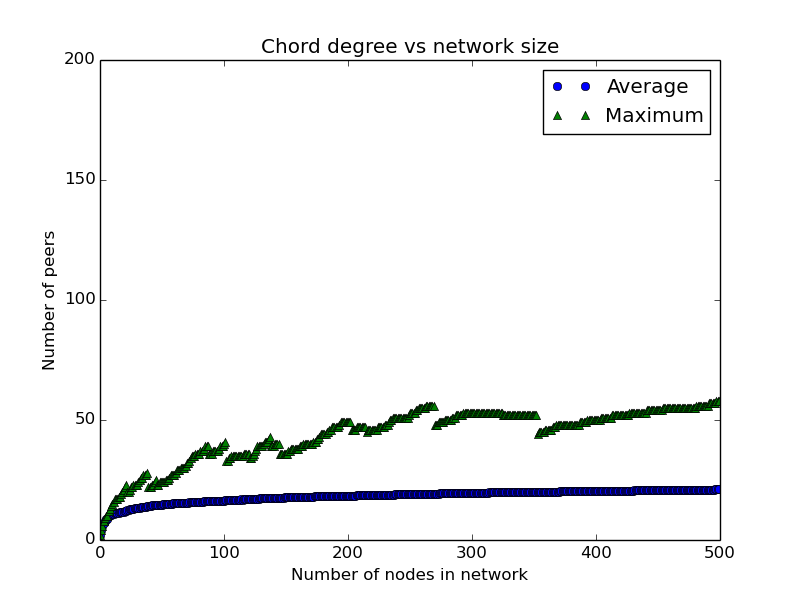
\includegraphics[width=\linewidth]{figs/ChordDegree}
	\caption{This is the average and maximum degree of nodes in the Chord network. This Chord network utilized a 120 bit hash and thus degree is bound at 122 (full fingers, predecessor and successor) when the network reaches $2^{120}$ nodes.}
	\label{fig:ChordDegree}
\end{figure}

\begin{figure}
	\centering
	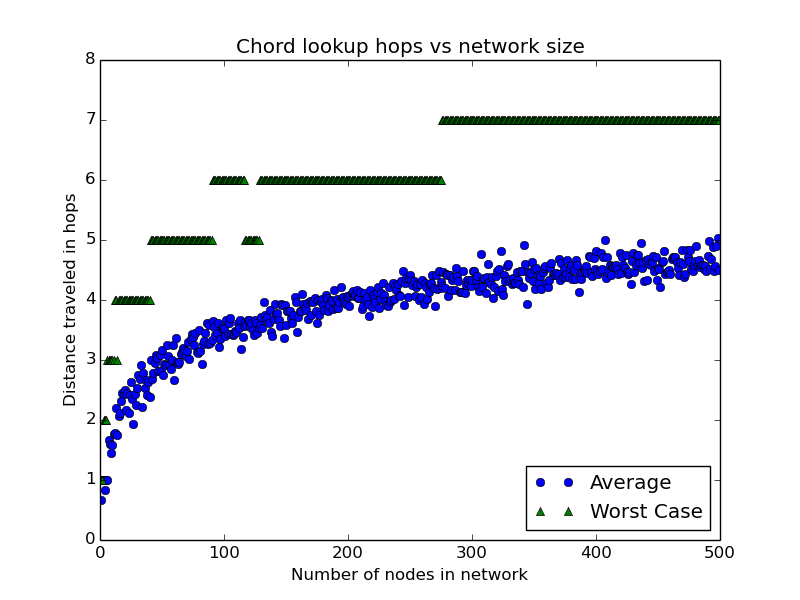
\includegraphics[width=\linewidth]{figs/ChordDistance}
	\caption{This is the number hops required for a greedy routed lookup in Chord. The average lookup between two nodes follows the expected logarithmic curve.}
	\label{fig:ChordDistance}
\end{figure}

\begin{figure}
	\centering
	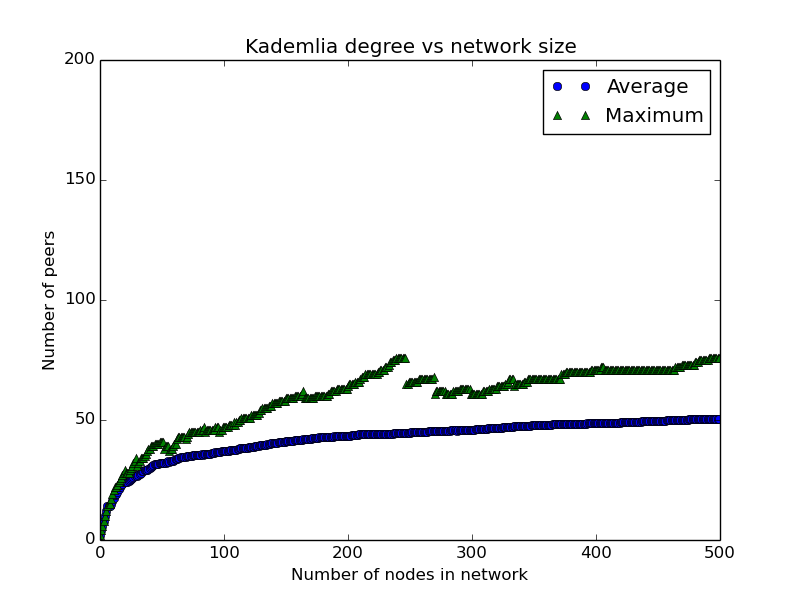
\includegraphics[width=\linewidth]{figs/KademliaDegree}
	\caption{This is the average and maximum degree of nodes in the Kademlia network as new nodes are added.  Both the maximum degree and average degree are $O(\log n)$.}
	\label{fig:KademliaDegree}
\end{figure}
\begin{figure}
	\centering
	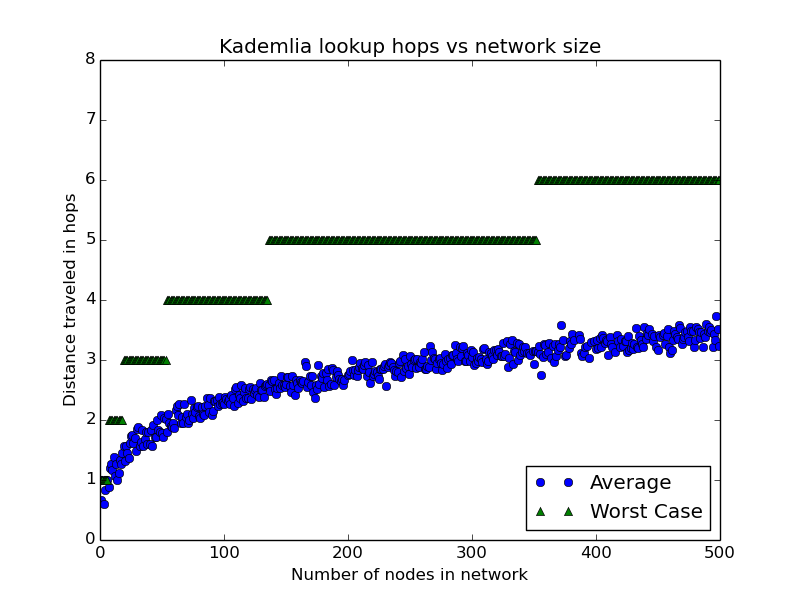
\includegraphics[width=\linewidth]{figs/KademliaDistance}
	\caption{Much like Chord, the average degree follows a distinct logarithmic curve, reaching an average distance of approximately three hops when there are 500 nodes in the network.}
	\label{fig:KademliaDistance}
\end{figure}



The results of our Euclidean and Hyperbolic geometries indicate similar asymptotic behavior: a higher degree produces a lower diameter and average routing. 
However, the ability to leverage this trade-off is limited by the necessity of maintaining an $ O(\log n $) degree.
These results are shown in Figures \ref{fig:EucldianDegree} - \ref{fig:HyperbolicDistance}.

While we maintain the number of links must be $ O(\log n)$, all DHTs practically bound this number by a constant.  
For example, in Chord, this is the number of bits in the hash function plus the number of predecessors/successors.
Chord and Kademlia fill this bound asymptotically. 
The long peer strategy used by the Euclidean and Hyperbolic metrics aggressively filled to this capacity, relying on the distribution of long peers to change as the network increased in size rather than increasing the number of utilized long peers.
This explains why the Euclidean and Hyperbolic spaces have more peers (and thus lower diameter) for a given network size.
This presents a strategy for trade-off of the network diameter vs. the overhead maintenance cost.


%\subsection{Chord}
%Our model of Chord
%\cite{chord}.


\begin{figure}
\centering
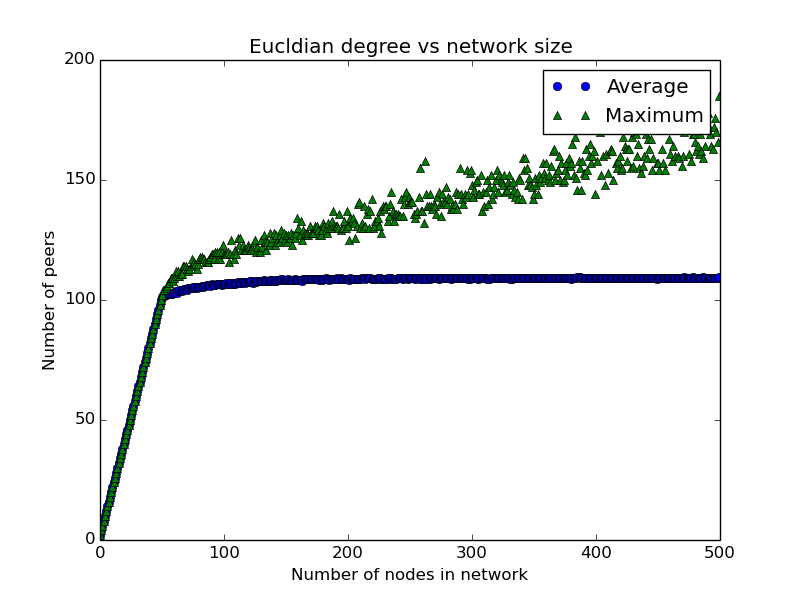
\includegraphics[width=\linewidth]{figs/EucldianDegree}
\caption{Because the long peers increase linearly to the maximum value (49), degree initially rises quickly and then grows  more slowly as the number of long peers ceases to grow and the size short peers increases with network size. }
\label{fig:EucldianDegree}
\end{figure}

\begin{figure}
\centering
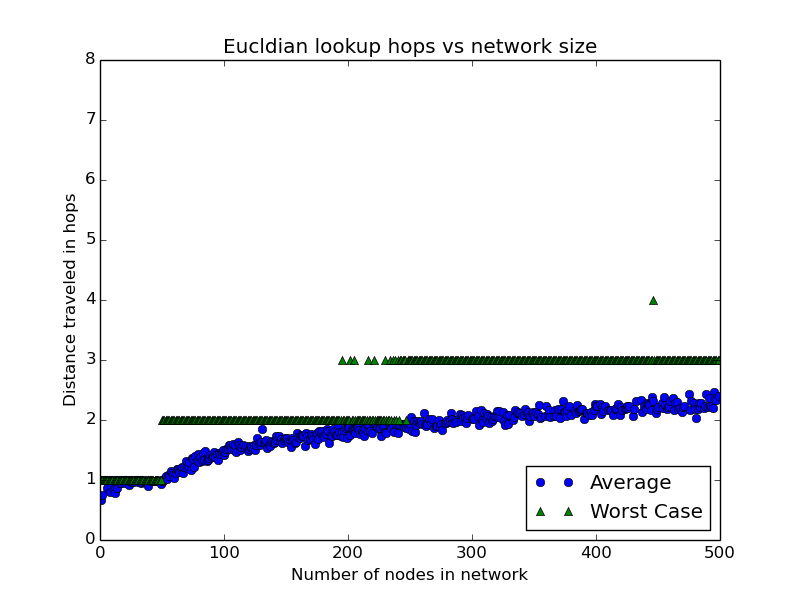
\includegraphics[width=\linewidth]{figs/EucldianDistance}
\caption{The inter-node distance stays constant at 1 until long peers are filled, then rises at the rate of a randomly connected network due to the distribution of long peers selected}
\label{fig:EucldianDistance}
\end{figure}

\begin{figure}
\centering
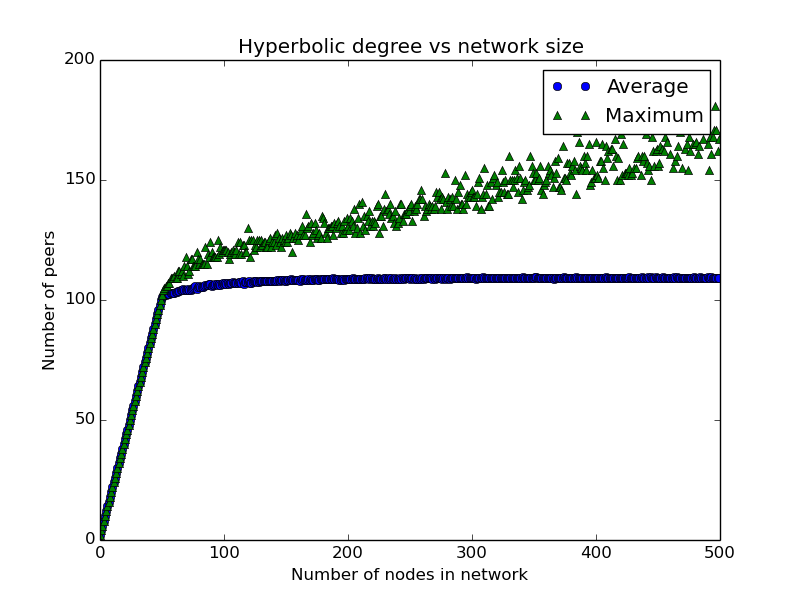
\includegraphics[width=\linewidth]{figs/HyperbolicDegree}
\caption{The Hyperbolic network uses the same long and short peer strategies to the Euclidean network, and thus shows similar results.}
\label{fig:HyperbolicDegree}
\end{figure}
\begin{figure}
\centering
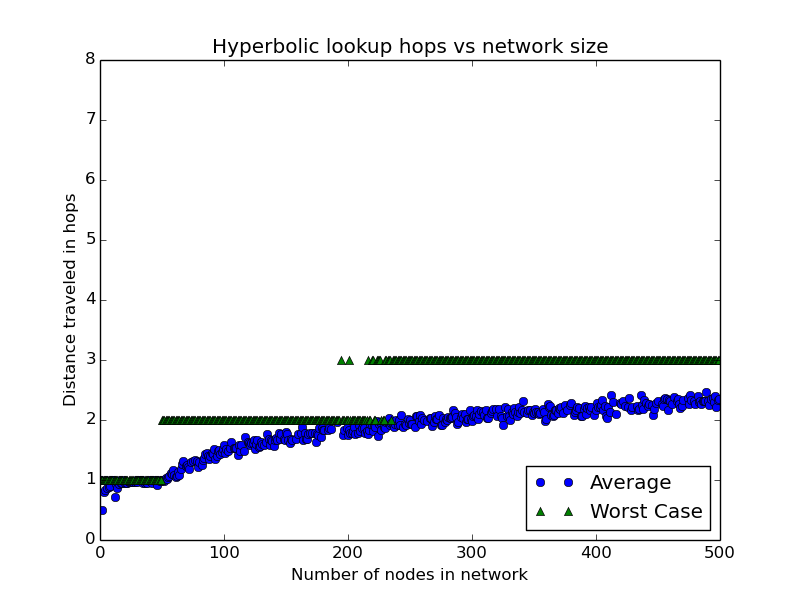
\includegraphics[width=\linewidth]{figs/HyperbolicDistance}
\caption{Like the Euclidean Geometry, our Poincar\`{e} disc based topology has much shorter maximum and average distances.
}
\label{fig:HyperbolicDistance}
\end{figure}


\section{Related Work}\label{sec:related}

There have been a number of efforts to either create abstractions of DHTs or ease the development of DHTs.
One area of previous work focused on constructing overlay networks using system called P2 \cite{p2} \cite{loo2005implementing}.
P2 is a network engine for constructing overlays which uses the Overlog declarative logic language.
Writing programs for P2 in Overlog yields extremely concise and modular implementations of for overlay networks. 

Our work differs in that P2 attempts to abstract overlays and ease construction by using a language and framework. while UrDHT focuses on abstracting the idea of a structured overlay into Voronoi Tessellations and Delaunay Triangulations.
This allows developers to define the overlays they are building by mathematically defining a short number of functions.

Our use case is also subtly different. 
P2 focuses on overlays in general, all types of overlays.
UrDHT concerns itself solely with distributed hash tables, specifically, overlays that rely on hash functions to distribute the load of the network and assign responsibility in an autonomous manner. 

One difficulty in using P2 is that it is no longer supported as a project \cite{p2}. 
P2's concise Overlog statements also present a sharp learning curve for many developers.
These present challenges not seen with UrDHT.


The T-Man\cite{jelasity2005t} and Vicinity \cite{voulgaris2005epidemic} protocols both present gossip-based methods for organizing overlay networks.
The idea behind T-Man is similar to UrDHT, but again it focuses on overlays in general, while UrDHT applies specifically to DHTs.
% T-man boasts the topology can change at run-time as the needs demand. 
The ranking function is similar to the metrics used by UrDHT using DGVH, but DGVH guarantees full connectivity in all cases and is based on the inherent relationship between Voronoi Tessellations, Delaunay Triangulations, and DHTs.

UrDHT uses a gossiping protocol similar to the ones presented by T-Man and Vicinity due to they gossip protocol's ability to rapidly adjust changes in the topology.


\section{Applications and Future Work}
\label{sec:future}

%Restate the intro
We presented UrDHT, a unified model for DHTs and framework for building distributed applications.
We have shown how it possible to use UrDHT to not only implement traditional DHTs such as Chord and Kademlia, but also in much more generalized spaces such as Euclidean and Hyperbolic geometries.
The viability of UrDHT to utilize Euclidean and Hyperbolic metric spaces indicates that further research into potential topologies of DHTs and potential applications of these topologies is warranted.


%Future improvements of UrDHT would further disconnect long peers and short peers giving them their own implementation cycle.

%Future stuff
There are numerous routes we can take with our model.
Of particular interest are the applications of building a DHT overlay that operates in a hyperbolic geometry.

One of the other features shared by nearly every DHT is that routing works by minimizing the number of hops across the overlay network, with all hops treated as the same length.
This is done because it is assumed that DHTs know nothing about the state of actual infrastructure the overlay is built upon.

However, this means that most DHTs could happily route a message from one continent to another and back.
This is obviously undesirable, but it is the status quo in DHTs.
The reason for this stems from the generation of node IDs in DHTs. 
Nodes are typically assigned a point in the range of a cryptographic hash function. 
The ID corresponds to the hash of some identifier or given a point randomly.
This is done for purposes of load balancing and fault tolerance.

For future work, we want to see if there is a means of embedding latency into the DHT, while still maintaining the system's fault tolerance.
Doing so would mean that the hops traversed to a destination are, in fact, the shortest path to the destination.

We believe we can embed a latency graph in a hyperbolic space and define UrDHT such that it operates within this space \cite{kleinberg2007geographic} \cite{cvetkovski2009hyperbolic}.
The end result would be a DHT with latency embedded into the overlay.
Nodes would respond to changes in latency and the network by rejoining the network at new positions.
This approach would maintain the decentralized strengths of DHTs, while reducing overall delay and communication costs.


\section{Remarks}
	
	\bibliography{notes,dht,mapreduce,voronoi,dns,botnets,mine}
	\bibliographystyle{plain}
\end{document}
